\chapter{Neural Networks}
\label{neural_networks}

In this part we describe how to define $\mathcal{H}$ using functions called \textbf{neural networks}. One advantage of these functions is that they're easy to adapt to multi-task learning. We begin by describing how to design $\mathcal{H}$ using neural networks. We then turn to the issue of how to use $\mathcal{D}$ to search this hypothesis space. We then cover regularization techniques, the purpose of which is to prevent overfitting. Lastly, we introduce convolutional neural networks which are specialized functions often used for text classification problems such as relation extraction.

\section{Feed-Forward Neural Networks}
A feed-forward neural network is a function $h: \mathcal{X} \mapsto \mathcal{Y}$. To understand how it works, it's instructive to look at each part of its name in isolation.
\\\\
$h$ is called a \textbf{network} because it's a composition of $L$ \textbf{layers} of other functions $f^{(l)}$. Each $f^{(l)}$ receives input from $f^{(l-1)}$. For example if $L = 2$, then $h(\mathbf{x}) = f^{(2)}(f^{(1)}(\mathbf{x}))$. We denote the input to $f^{(1)}$ as $\mathbf{x}^{(0)}$, which is identical to the input vector $\mathbf{x}$, except for an added \textbf{bias} component of 1, as described later in this section. each $f^{(l)}$ outputs a vector $\mathbf{x}^{(l)}$ of dimension $d^{(l)}$ which is the input of $f^{(l+1)}$. The dimensionality of these vectors determine the \textbf{width} of the network. The number of layers $L$ is called the \textbf{depth} of the network. $f^{(L)}$ is called the \textbf{output layer}. The remaining functions $f^{(1)}$ to $f^{(L-1)}$ are called \textbf{hidden layers}. 
\\\\
The functions $f^{(1)}$ to $f^{(L)}$ are ordered by their index $l$. By ordered, we mean that the index of the innermost functions are smaller than the index of the outermost. $h$ is called a \textbf{feed-forward} network because each $f^{(l)}$ can receive input only from functions $f^{(i)}$ if $l > i$. In other words, it's not possible for a function $f^{(l)}$ to feed its own output into itself, or any other function that it receives input from.
\\\\
Finally $h$ is called a \textbf{neural} network since its design is loosely based on neurons in the brain \citep{goodfellow16}. Each component $x_i$ of the vector $\mathbf{x}^{(l)}$ can be seen as the output of a unit similar to a neuron. Each unit in layer $l$ receives input from units in layer $l-1$. The output $x^{(l-1)}_i$ of unit $i$ in layer $l-1$ is multiplied by a weight $w^{(l)}_{ij}$ that gives the strength of the connection between unit $i$ in $l-1$ and unit $j$ in $l$. Unit $j$ sums all of the input it receives from units in layer $l-1$ to obtain its \textbf{activation} $a^{(l)}_j = \sum_{i=0}^{d^{(l-1)}} w^{(l)}_{ij}x^{(l-1)}_{i}$. To compute its output $x^{(l)}_j$, it applies an \textbf{activation function} $\sigma(a^{(l)}_j)$ to its activation.

Activation functions model the behaviour of biological neurons by outputting a signal only when the activation is above a certain threshold. To make it possible to learn this threshold for each unit using the same activation function, we introduce a special \textbf{bias} unit that always outputs 1. The index of the bias unit in layer $l$ is 0 by convention. Figure \ref{connection}. shows how a unit $j$ computes its output $x^{(l)}_j$ by combining the outputs of units in layer $l-1$.

\tikzstyle{neuron}=[circle,draw,minimum size=20pt,inner sep=0pt]
\tikzstyle{summation} = [square, minimum size=20pt,inner sep=0pt]
\tikzstyle{edge} = [draw,thick,-]
\tikzstyle{weight} = [font=\small]

\begin{figure}[h]
	\centering
	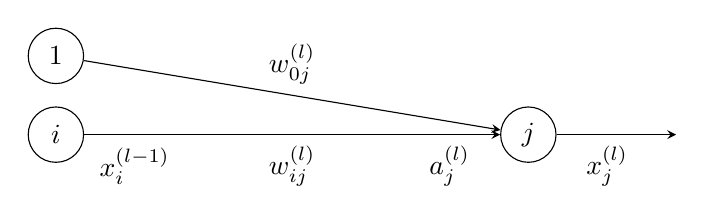
\begin{tikzpicture}[->, >=stealth, swap]
			\node [neuron] (sigma1) at (0,0) {$i$};
			\node [neuron] (sigma2) at (6,0) {$j$};
			\node [neuron] (bias1) at (0,1) {$1$};
			\node []       (z1)      at (1,-.4) {$x^{(l-1)}_i$};
			\node []       (w)     at (3,-.4) {$w^{(l)}_{ij}$};
			\node []       (w)     at (3,.9) {$w^{(l)}_{0j}$};
			\node []       (aw)   at (5,-.4) {$a^{(l)}_j$};
			\node []	   (empty) at (8,0) {};
			\node []       (z2)    at (7,-.4) {$x^{(l)}_j$};
		
			\draw (sigma1) edge (sigma2);
			\draw (sigma2) edge (empty);
			\draw (bias1) edge (sigma2);
	\end{tikzpicture}
	\caption{A visual representation of the connections between unit $i$ in layer $l-1$, the bias unit in $l-1$, and unit $j$ in layer $l$. The connection strength between these units is given by the weight $w^{(l)}_{ij}$ between $i$ and $j$, and $w^{(l)}_{0j}$ between the bias unit and $j$. The activation $a^{(l)}_j$ at unit $j$ is computed by $a^{(l)}_j = w^{(l)}_{ij}x^{(l)}_i + w^{(l)}_0$. The output $x^{(l)}_j$ of unit $j$ is given by $x^{(l)}_j = \sigma(a^{(l)}_j)$}
	\label{connection}
\end{figure}
\noindent
Keeping track of the indices $l$, $i$ and $j$ quickly becomes confusing. By collecting all of the weights of connections going into unit $j$ in layer $l$ in a vector $\mathbf{w}^{(l)}_j$, the activation at unit $j$ can be computed as a dot product $a^{(l)}_j = {\mathbf{w}^{(l)}_j} \cdot \mathbf{x}^{(l-1)}$. Moreover, we can compute the entire vector $\mathbf{a}^{(l)}$ of activations at layer $l$, by organising the weight vectors $\mathbf{w}^{(l)}_j$ in a matrix $\mathbf{W}^{(l)} = \begin{bmatrix} \mathbf{w}^{(l)}_1 & \dots & \mathbf{w}^{(l)}_{d^{(l)}} \end{bmatrix}^T$, which leads to $\mathbf{a}^{(l)} = \mathbf{W}^{(l)}\mathbf{x}^{(l-1)}$.
\\\\
By gathering the weights in matrices $\mathbf{W}^{(l)}$, we have simplified our view of $h$ into a composition of matrix-vector products and element-wise application of activation functions. Figure \ref{neural_network} shows the parallel views of neural networks as networks of units and matrix-vector operations.

\begin{figure}[h]
	\centering
	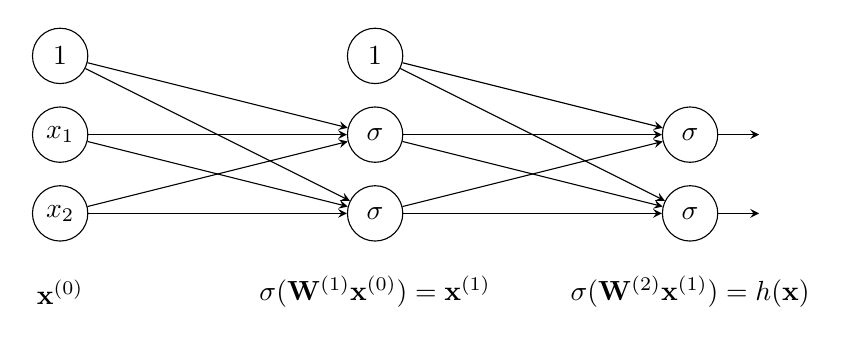
\begin{tikzpicture}[->, >=stealth, swap]
		\node [neuron] (bias0)   at (0, 2)  {1};
		\node [neuron] (x1)      at (0, 1)  {$x_1$};
		\node [neuron] (x2)      at (0, 0)  {$x_2$};
		\node []       (x)       at (0,-1)  {$\mathbf{x}^{(0)}$};
		\node [neuron] (bias1)   at (4, 2)  {1}; 
		\node [neuron] (sigma11) at (4, 1)  {$\sigma$};
		\node [neuron] (sigma12) at (4, 0)  {$\sigma$};
		\node []       (layer1)  at (4,-1)  {$\sigma(\mathbf{W}^{(1)} \mathbf{x}^{(0)}) = \mathbf{x}^{(1)}$};
		\node [neuron] (sigma21) at (8, 1)  {$\sigma$};
		\node [neuron] (sigma22) at (8, 0)  {$\sigma$};
		\node []       (layer2)  at (8,-1)  {$\sigma(\mathbf{W}^{(2)} \mathbf{x}^{(1)}) = h(\mathbf{x})$};
		\node []	   (empty1)  at (9, 1) {};
		\node []       (empty2)  at (9, 0) {};   
		
		
		\draw (bias0)   edge (sigma11);
		\draw (x1)      edge (sigma11);
		\draw (x2)      edge (sigma11);
		\draw (bias0)   edge (sigma12);
		\draw (x1)      edge (sigma12);
		\draw (x2)      edge (sigma12);
		\draw (bias1)   edge (sigma21);
		\draw (sigma11) edge (sigma21);
		\draw (sigma12) edge (sigma21);
		\draw (bias1)   edge (sigma22);
		\draw (sigma11) edge (sigma22);
		\draw (sigma12) edge (sigma22);
		\draw (sigma21) edge (empty1);
		\draw (sigma22) edge (empty2);
	\end{tikzpicture}
	\caption{A visual representation of $h(\mathbf{x}) = f_2(f_1(\mathbf{x}^{(0)}))$. The activation at each layer $\mathbf{a}^{(l)}$ is computed by $\mathbf{W}^{(l)}\mathbf{x}^{(l-1)}$. The output at each layer is computed by element-wise application of the activation function of $\sigma(\mathbf{a}^{(l)})$.}
	\label{neural_network}
\end{figure}
\noindent
We now have all the components we need to specify $\mathcal{H}$ as a set of neural networks. The set is defined by the depth of the networks $L$, the number of units in each layer $d_l$ , and the activation function $\sigma$.
For a particular $L$, $d_l$, and $\sigma$, each $h \in \mathcal{H}$ corresponds exactly to a unique assignment of real numbers to all of its weights. We can make the dependence of $h$ on its weights explicit by defining a vector $\mathbf{w} = \begin{bmatrix} w^{(1)}_{ij} & \dots & w^{(L)}_{ij}\end{bmatrix}$ and writing $h(\mathbf{x}, \mathbf{w})$ which means \textit{the function $h$ parameterised by the weight vector $\mathbf{w}$}. In the next section we discuss how to choose the activation functions at the layers of the network.

\subsection{Activation Functions}
\label{activation_functions}
Activation functions mimic the behaviour of neurons in the brain. A neuron emits a signal when the combined input it receives from other neurons exceeds a certain threshold. Activation functions achieve this by a variation of the step function, where an activation signal $a^{(l)}_j$ below the threshold is mapped to a value near zero, and an activation signal above the threshold is mapped to a value greater than zero. From a mathematical perspective, the role of activation functions is to introduce non-linearity in $h$, which allows it to approximate a much larger class of functions.
\\\\
Many networks use \textbf{sigmoid} activation functions such as the classical sigmoid function $\sigma(a) = \frac{1}{1 + \me^-a}$. These functions have the advantage of being differentiable everywhere. As we will see in section \ref{learning_algorithm}, differential calculus is the fundamental tool for finding a good $h \in \mathcal{H}$, which makes differentiability a desirable quality. One drawback of sigmoid activation functions is that their derivates are small, as seen in figure \ref{sigmoid}. For example, we can show that $\max \frac{d\sigma}{da} = \frac{1}{4}$. As we will see in section \ref{learning_algorithm}, neural networks are trained by multiplying chains of derivatives. When these derivatives are smaller than 1, the magnitude of the derivative shrinks in the length of the chain of terms which can make learning from $\mathcal{D}_{train}$ extremely slow.
\begin{figure}
	\centering
	%% Creator: Matplotlib, PGF backend
%%
%% To include the figure in your LaTeX document, write
%%   \input{<filename>.pgf}
%%
%% Make sure the required packages are loaded in your preamble
%%   \usepackage{pgf}
%%
%% Figures using additional raster images can only be included by \input if
%% they are in the same directory as the main LaTeX file. For loading figures
%% from other directories you can use the `import` package
%%   \usepackage{import}
%% and then include the figures with
%%   \import{<path to file>}{<filename>.pgf}
%%
%% Matplotlib used the following preamble
%%   \usepackage{fontspec}
%%   \setmainfont{Palatino}
%%   \setsansfont{Lucida Grande}
%%   \setmonofont{Andale Mono}
%%
\begingroup%
\makeatletter%
\begin{pgfpicture}%
\pgfpathrectangle{\pgfpointorigin}{\pgfqpoint{4.614828in}{3.237168in}}%
\pgfusepath{use as bounding box, clip}%
\begin{pgfscope}%
\pgfsetbuttcap%
\pgfsetmiterjoin%
\definecolor{currentfill}{rgb}{1.000000,1.000000,1.000000}%
\pgfsetfillcolor{currentfill}%
\pgfsetlinewidth{0.000000pt}%
\definecolor{currentstroke}{rgb}{1.000000,1.000000,1.000000}%
\pgfsetstrokecolor{currentstroke}%
\pgfsetdash{}{0pt}%
\pgfpathmoveto{\pgfqpoint{0.000000in}{-0.000000in}}%
\pgfpathlineto{\pgfqpoint{4.614828in}{-0.000000in}}%
\pgfpathlineto{\pgfqpoint{4.614828in}{3.237168in}}%
\pgfpathlineto{\pgfqpoint{0.000000in}{3.237168in}}%
\pgfpathclose%
\pgfusepath{fill}%
\end{pgfscope}%
\begin{pgfscope}%
\pgfsetbuttcap%
\pgfsetmiterjoin%
\definecolor{currentfill}{rgb}{1.000000,1.000000,1.000000}%
\pgfsetfillcolor{currentfill}%
\pgfsetlinewidth{0.000000pt}%
\definecolor{currentstroke}{rgb}{0.000000,0.000000,0.000000}%
\pgfsetstrokecolor{currentstroke}%
\pgfsetstrokeopacity{0.000000}%
\pgfsetdash{}{0pt}%
\pgfpathmoveto{\pgfqpoint{0.074056in}{0.375732in}}%
\pgfpathlineto{\pgfqpoint{4.559273in}{0.375732in}}%
\pgfpathlineto{\pgfqpoint{4.559273in}{3.237168in}}%
\pgfpathlineto{\pgfqpoint{0.074056in}{3.237168in}}%
\pgfpathclose%
\pgfusepath{fill}%
\end{pgfscope}%
\begin{pgfscope}%
\pgfpathrectangle{\pgfqpoint{0.074056in}{0.375732in}}{\pgfqpoint{4.485217in}{2.861436in}} %
\pgfusepath{clip}%
\pgfsetrectcap%
\pgfsetroundjoin%
\pgfsetlinewidth{1.003750pt}%
\definecolor{currentstroke}{rgb}{0.000000,0.000000,1.000000}%
\pgfsetstrokecolor{currentstroke}%
\pgfsetdash{}{0pt}%
\pgfpathmoveto{\pgfqpoint{0.074056in}{0.375850in}}%
\pgfpathlineto{\pgfqpoint{0.522578in}{0.376604in}}%
\pgfpathlineto{\pgfqpoint{0.724412in}{0.377877in}}%
\pgfpathlineto{\pgfqpoint{0.858969in}{0.379637in}}%
\pgfpathlineto{\pgfqpoint{0.971099in}{0.382164in}}%
\pgfpathlineto{\pgfqpoint{1.060804in}{0.385316in}}%
\pgfpathlineto{\pgfqpoint{1.128082in}{0.388652in}}%
\pgfpathlineto{\pgfqpoint{1.195360in}{0.393142in}}%
\pgfpathlineto{\pgfqpoint{1.240212in}{0.396965in}}%
\pgfpathlineto{\pgfqpoint{1.285064in}{0.401620in}}%
\pgfpathlineto{\pgfqpoint{1.329917in}{0.407282in}}%
\pgfpathlineto{\pgfqpoint{1.374769in}{0.414164in}}%
\pgfpathlineto{\pgfqpoint{1.419621in}{0.422520in}}%
\pgfpathlineto{\pgfqpoint{1.464473in}{0.432652in}}%
\pgfpathlineto{\pgfqpoint{1.486899in}{0.438494in}}%
\pgfpathlineto{\pgfqpoint{1.509325in}{0.444919in}}%
\pgfpathlineto{\pgfqpoint{1.531751in}{0.451982in}}%
\pgfpathlineto{\pgfqpoint{1.554177in}{0.459742in}}%
\pgfpathlineto{\pgfqpoint{1.576604in}{0.468263in}}%
\pgfpathlineto{\pgfqpoint{1.599030in}{0.477614in}}%
\pgfpathlineto{\pgfqpoint{1.621456in}{0.487867in}}%
\pgfpathlineto{\pgfqpoint{1.643882in}{0.499101in}}%
\pgfpathlineto{\pgfqpoint{1.666308in}{0.511399in}}%
\pgfpathlineto{\pgfqpoint{1.688734in}{0.524850in}}%
\pgfpathlineto{\pgfqpoint{1.711160in}{0.539545in}}%
\pgfpathlineto{\pgfqpoint{1.733586in}{0.555582in}}%
\pgfpathlineto{\pgfqpoint{1.756012in}{0.573062in}}%
\pgfpathlineto{\pgfqpoint{1.778438in}{0.592090in}}%
\pgfpathlineto{\pgfqpoint{1.800864in}{0.612771in}}%
\pgfpathlineto{\pgfqpoint{1.823290in}{0.635213in}}%
\pgfpathlineto{\pgfqpoint{1.845717in}{0.659526in}}%
\pgfpathlineto{\pgfqpoint{1.868143in}{0.685815in}}%
\pgfpathlineto{\pgfqpoint{1.890569in}{0.714184in}}%
\pgfpathlineto{\pgfqpoint{1.912995in}{0.744730in}}%
\pgfpathlineto{\pgfqpoint{1.935421in}{0.777543in}}%
\pgfpathlineto{\pgfqpoint{1.957847in}{0.812703in}}%
\pgfpathlineto{\pgfqpoint{1.980273in}{0.850276in}}%
\pgfpathlineto{\pgfqpoint{2.002699in}{0.890312in}}%
\pgfpathlineto{\pgfqpoint{2.025125in}{0.932841in}}%
\pgfpathlineto{\pgfqpoint{2.047551in}{0.977870in}}%
\pgfpathlineto{\pgfqpoint{2.069977in}{1.025382in}}%
\pgfpathlineto{\pgfqpoint{2.092403in}{1.075331in}}%
\pgfpathlineto{\pgfqpoint{2.114830in}{1.127641in}}%
\pgfpathlineto{\pgfqpoint{2.137256in}{1.182203in}}%
\pgfpathlineto{\pgfqpoint{2.159682in}{1.238877in}}%
\pgfpathlineto{\pgfqpoint{2.182108in}{1.297488in}}%
\pgfpathlineto{\pgfqpoint{2.226960in}{1.419668in}}%
\pgfpathlineto{\pgfqpoint{2.271812in}{1.546751in}}%
\pgfpathlineto{\pgfqpoint{2.406369in}{1.933102in}}%
\pgfpathlineto{\pgfqpoint{2.451221in}{2.055281in}}%
\pgfpathlineto{\pgfqpoint{2.473647in}{2.113893in}}%
\pgfpathlineto{\pgfqpoint{2.496073in}{2.170566in}}%
\pgfpathlineto{\pgfqpoint{2.518499in}{2.225129in}}%
\pgfpathlineto{\pgfqpoint{2.540925in}{2.277439in}}%
\pgfpathlineto{\pgfqpoint{2.563351in}{2.327388in}}%
\pgfpathlineto{\pgfqpoint{2.585777in}{2.374900in}}%
\pgfpathlineto{\pgfqpoint{2.608203in}{2.419929in}}%
\pgfpathlineto{\pgfqpoint{2.630629in}{2.462457in}}%
\pgfpathlineto{\pgfqpoint{2.653056in}{2.502493in}}%
\pgfpathlineto{\pgfqpoint{2.675482in}{2.540066in}}%
\pgfpathlineto{\pgfqpoint{2.697908in}{2.575226in}}%
\pgfpathlineto{\pgfqpoint{2.720334in}{2.608040in}}%
\pgfpathlineto{\pgfqpoint{2.742760in}{2.638586in}}%
\pgfpathlineto{\pgfqpoint{2.765186in}{2.666954in}}%
\pgfpathlineto{\pgfqpoint{2.787612in}{2.693243in}}%
\pgfpathlineto{\pgfqpoint{2.810038in}{2.717556in}}%
\pgfpathlineto{\pgfqpoint{2.832464in}{2.739999in}}%
\pgfpathlineto{\pgfqpoint{2.854890in}{2.760680in}}%
\pgfpathlineto{\pgfqpoint{2.877316in}{2.779707in}}%
\pgfpathlineto{\pgfqpoint{2.899742in}{2.797187in}}%
\pgfpathlineto{\pgfqpoint{2.922168in}{2.813225in}}%
\pgfpathlineto{\pgfqpoint{2.944595in}{2.827920in}}%
\pgfpathlineto{\pgfqpoint{2.967021in}{2.841370in}}%
\pgfpathlineto{\pgfqpoint{2.989447in}{2.853668in}}%
\pgfpathlineto{\pgfqpoint{3.011873in}{2.864902in}}%
\pgfpathlineto{\pgfqpoint{3.034299in}{2.875156in}}%
\pgfpathlineto{\pgfqpoint{3.056725in}{2.884506in}}%
\pgfpathlineto{\pgfqpoint{3.079151in}{2.893027in}}%
\pgfpathlineto{\pgfqpoint{3.101577in}{2.900787in}}%
\pgfpathlineto{\pgfqpoint{3.124003in}{2.907851in}}%
\pgfpathlineto{\pgfqpoint{3.146429in}{2.914276in}}%
\pgfpathlineto{\pgfqpoint{3.191281in}{2.925427in}}%
\pgfpathlineto{\pgfqpoint{3.236134in}{2.934630in}}%
\pgfpathlineto{\pgfqpoint{3.280986in}{2.942214in}}%
\pgfpathlineto{\pgfqpoint{3.325838in}{2.948457in}}%
\pgfpathlineto{\pgfqpoint{3.370690in}{2.953591in}}%
\pgfpathlineto{\pgfqpoint{3.415542in}{2.957810in}}%
\pgfpathlineto{\pgfqpoint{3.482821in}{2.962766in}}%
\pgfpathlineto{\pgfqpoint{3.550099in}{2.966450in}}%
\pgfpathlineto{\pgfqpoint{3.639803in}{2.969931in}}%
\pgfpathlineto{\pgfqpoint{3.729507in}{2.972270in}}%
\pgfpathlineto{\pgfqpoint{3.841638in}{2.974144in}}%
\pgfpathlineto{\pgfqpoint{3.998620in}{2.975600in}}%
\pgfpathlineto{\pgfqpoint{4.245307in}{2.976559in}}%
\pgfpathlineto{\pgfqpoint{4.536846in}{2.976907in}}%
\pgfpathlineto{\pgfqpoint{4.536846in}{2.976907in}}%
\pgfusepath{stroke}%
\end{pgfscope}%
\begin{pgfscope}%
\pgfpathrectangle{\pgfqpoint{0.074056in}{0.375732in}}{\pgfqpoint{4.485217in}{2.861436in}} %
\pgfusepath{clip}%
\pgfsetrectcap%
\pgfsetroundjoin%
\pgfsetlinewidth{1.003750pt}%
\definecolor{currentstroke}{rgb}{0.000000,0.500000,0.000000}%
\pgfsetstrokecolor{currentstroke}%
\pgfsetdash{}{0pt}%
\pgfpathmoveto{\pgfqpoint{0.074056in}{0.375850in}}%
\pgfpathlineto{\pgfqpoint{0.522578in}{0.376604in}}%
\pgfpathlineto{\pgfqpoint{0.724412in}{0.377875in}}%
\pgfpathlineto{\pgfqpoint{0.858969in}{0.379631in}}%
\pgfpathlineto{\pgfqpoint{0.971099in}{0.382148in}}%
\pgfpathlineto{\pgfqpoint{1.060804in}{0.385280in}}%
\pgfpathlineto{\pgfqpoint{1.128082in}{0.388588in}}%
\pgfpathlineto{\pgfqpoint{1.195360in}{0.393026in}}%
\pgfpathlineto{\pgfqpoint{1.240212in}{0.396792in}}%
\pgfpathlineto{\pgfqpoint{1.285064in}{0.401362in}}%
\pgfpathlineto{\pgfqpoint{1.329917in}{0.406899in}}%
\pgfpathlineto{\pgfqpoint{1.374769in}{0.413596in}}%
\pgfpathlineto{\pgfqpoint{1.419621in}{0.421678in}}%
\pgfpathlineto{\pgfqpoint{1.464473in}{0.431406in}}%
\pgfpathlineto{\pgfqpoint{1.509325in}{0.443079in}}%
\pgfpathlineto{\pgfqpoint{1.531751in}{0.449747in}}%
\pgfpathlineto{\pgfqpoint{1.554177in}{0.457029in}}%
\pgfpathlineto{\pgfqpoint{1.576604in}{0.464972in}}%
\pgfpathlineto{\pgfqpoint{1.599030in}{0.473624in}}%
\pgfpathlineto{\pgfqpoint{1.621456in}{0.483033in}}%
\pgfpathlineto{\pgfqpoint{1.643882in}{0.493250in}}%
\pgfpathlineto{\pgfqpoint{1.666308in}{0.504324in}}%
\pgfpathlineto{\pgfqpoint{1.688734in}{0.516302in}}%
\pgfpathlineto{\pgfqpoint{1.711160in}{0.529229in}}%
\pgfpathlineto{\pgfqpoint{1.733586in}{0.543148in}}%
\pgfpathlineto{\pgfqpoint{1.756012in}{0.558093in}}%
\pgfpathlineto{\pgfqpoint{1.778438in}{0.574095in}}%
\pgfpathlineto{\pgfqpoint{1.800864in}{0.591171in}}%
\pgfpathlineto{\pgfqpoint{1.823290in}{0.609330in}}%
\pgfpathlineto{\pgfqpoint{1.845717in}{0.628565in}}%
\pgfpathlineto{\pgfqpoint{1.868143in}{0.648852in}}%
\pgfpathlineto{\pgfqpoint{1.890569in}{0.670148in}}%
\pgfpathlineto{\pgfqpoint{1.912995in}{0.692387in}}%
\pgfpathlineto{\pgfqpoint{1.957847in}{0.739300in}}%
\pgfpathlineto{\pgfqpoint{2.002699in}{0.788520in}}%
\pgfpathlineto{\pgfqpoint{2.069977in}{0.863138in}}%
\pgfpathlineto{\pgfqpoint{2.092403in}{0.887180in}}%
\pgfpathlineto{\pgfqpoint{2.114830in}{0.910301in}}%
\pgfpathlineto{\pgfqpoint{2.137256in}{0.932176in}}%
\pgfpathlineto{\pgfqpoint{2.159682in}{0.952475in}}%
\pgfpathlineto{\pgfqpoint{2.182108in}{0.970870in}}%
\pgfpathlineto{\pgfqpoint{2.204534in}{0.987048in}}%
\pgfpathlineto{\pgfqpoint{2.226960in}{1.000724in}}%
\pgfpathlineto{\pgfqpoint{2.249386in}{1.011643in}}%
\pgfpathlineto{\pgfqpoint{2.271812in}{1.019598in}}%
\pgfpathlineto{\pgfqpoint{2.294238in}{1.024435in}}%
\pgfpathlineto{\pgfqpoint{2.316664in}{1.026058in}}%
\pgfpathlineto{\pgfqpoint{2.339090in}{1.024435in}}%
\pgfpathlineto{\pgfqpoint{2.361516in}{1.019598in}}%
\pgfpathlineto{\pgfqpoint{2.383943in}{1.011643in}}%
\pgfpathlineto{\pgfqpoint{2.406369in}{1.000724in}}%
\pgfpathlineto{\pgfqpoint{2.428795in}{0.987048in}}%
\pgfpathlineto{\pgfqpoint{2.451221in}{0.970870in}}%
\pgfpathlineto{\pgfqpoint{2.473647in}{0.952475in}}%
\pgfpathlineto{\pgfqpoint{2.496073in}{0.932176in}}%
\pgfpathlineto{\pgfqpoint{2.518499in}{0.910301in}}%
\pgfpathlineto{\pgfqpoint{2.540925in}{0.887180in}}%
\pgfpathlineto{\pgfqpoint{2.585777in}{0.838490in}}%
\pgfpathlineto{\pgfqpoint{2.675482in}{0.739300in}}%
\pgfpathlineto{\pgfqpoint{2.720334in}{0.692387in}}%
\pgfpathlineto{\pgfqpoint{2.742760in}{0.670148in}}%
\pgfpathlineto{\pgfqpoint{2.765186in}{0.648852in}}%
\pgfpathlineto{\pgfqpoint{2.787612in}{0.628565in}}%
\pgfpathlineto{\pgfqpoint{2.810038in}{0.609330in}}%
\pgfpathlineto{\pgfqpoint{2.832464in}{0.591171in}}%
\pgfpathlineto{\pgfqpoint{2.854890in}{0.574095in}}%
\pgfpathlineto{\pgfqpoint{2.877316in}{0.558093in}}%
\pgfpathlineto{\pgfqpoint{2.899742in}{0.543148in}}%
\pgfpathlineto{\pgfqpoint{2.922168in}{0.529229in}}%
\pgfpathlineto{\pgfqpoint{2.944595in}{0.516302in}}%
\pgfpathlineto{\pgfqpoint{2.967021in}{0.504324in}}%
\pgfpathlineto{\pgfqpoint{2.989447in}{0.493250in}}%
\pgfpathlineto{\pgfqpoint{3.011873in}{0.483033in}}%
\pgfpathlineto{\pgfqpoint{3.034299in}{0.473624in}}%
\pgfpathlineto{\pgfqpoint{3.056725in}{0.464972in}}%
\pgfpathlineto{\pgfqpoint{3.079151in}{0.457029in}}%
\pgfpathlineto{\pgfqpoint{3.101577in}{0.449747in}}%
\pgfpathlineto{\pgfqpoint{3.146429in}{0.436979in}}%
\pgfpathlineto{\pgfqpoint{3.191281in}{0.426319in}}%
\pgfpathlineto{\pgfqpoint{3.236134in}{0.417448in}}%
\pgfpathlineto{\pgfqpoint{3.280986in}{0.410089in}}%
\pgfpathlineto{\pgfqpoint{3.325838in}{0.403998in}}%
\pgfpathlineto{\pgfqpoint{3.370690in}{0.398967in}}%
\pgfpathlineto{\pgfqpoint{3.415542in}{0.394817in}}%
\pgfpathlineto{\pgfqpoint{3.482821in}{0.389925in}}%
\pgfpathlineto{\pgfqpoint{3.550099in}{0.386277in}}%
\pgfpathlineto{\pgfqpoint{3.639803in}{0.382819in}}%
\pgfpathlineto{\pgfqpoint{3.729507in}{0.380491in}}%
\pgfpathlineto{\pgfqpoint{3.841638in}{0.378623in}}%
\pgfpathlineto{\pgfqpoint{3.998620in}{0.377169in}}%
\pgfpathlineto{\pgfqpoint{4.245307in}{0.376211in}}%
\pgfpathlineto{\pgfqpoint{4.536846in}{0.375862in}}%
\pgfpathlineto{\pgfqpoint{4.536846in}{0.375862in}}%
\pgfusepath{stroke}%
\end{pgfscope}%
\begin{pgfscope}%
\pgfsetrectcap%
\pgfsetmiterjoin%
\pgfsetlinewidth{0.501875pt}%
\definecolor{currentstroke}{rgb}{0.000000,0.000000,0.000000}%
\pgfsetstrokecolor{currentstroke}%
\pgfsetdash{}{0pt}%
\pgfpathmoveto{\pgfqpoint{0.074056in}{0.375732in}}%
\pgfpathlineto{\pgfqpoint{4.559273in}{0.375732in}}%
\pgfusepath{stroke}%
\end{pgfscope}%
\begin{pgfscope}%
\pgfsetrectcap%
\pgfsetmiterjoin%
\pgfsetlinewidth{0.501875pt}%
\definecolor{currentstroke}{rgb}{0.000000,0.000000,0.000000}%
\pgfsetstrokecolor{currentstroke}%
\pgfsetdash{}{0pt}%
\pgfpathmoveto{\pgfqpoint{2.316664in}{0.375732in}}%
\pgfpathlineto{\pgfqpoint{2.316664in}{3.237168in}}%
\pgfusepath{stroke}%
\end{pgfscope}%
\begin{pgfscope}%
\pgfsetbuttcap%
\pgfsetroundjoin%
\definecolor{currentfill}{rgb}{0.000000,0.000000,0.000000}%
\pgfsetfillcolor{currentfill}%
\pgfsetlinewidth{0.501875pt}%
\definecolor{currentstroke}{rgb}{0.000000,0.000000,0.000000}%
\pgfsetstrokecolor{currentstroke}%
\pgfsetdash{}{0pt}%
\pgfsys@defobject{currentmarker}{\pgfqpoint{0.000000in}{0.000000in}}{\pgfqpoint{0.000000in}{0.055556in}}{%
\pgfpathmoveto{\pgfqpoint{0.000000in}{0.000000in}}%
\pgfpathlineto{\pgfqpoint{0.000000in}{0.055556in}}%
\pgfusepath{stroke,fill}%
}%
\begin{pgfscope}%
\pgfsys@transformshift{0.074056in}{0.375732in}%
\pgfsys@useobject{currentmarker}{}%
\end{pgfscope}%
\end{pgfscope}%
\begin{pgfscope}%
\pgftext[x=0.074056in,y=0.320176in,,top]{\rmfamily\fontsize{8.000000}{9.600000}\selectfont -10}%
\end{pgfscope}%
\begin{pgfscope}%
\pgfsetbuttcap%
\pgfsetroundjoin%
\definecolor{currentfill}{rgb}{0.000000,0.000000,0.000000}%
\pgfsetfillcolor{currentfill}%
\pgfsetlinewidth{0.501875pt}%
\definecolor{currentstroke}{rgb}{0.000000,0.000000,0.000000}%
\pgfsetstrokecolor{currentstroke}%
\pgfsetdash{}{0pt}%
\pgfsys@defobject{currentmarker}{\pgfqpoint{0.000000in}{0.000000in}}{\pgfqpoint{0.000000in}{0.055556in}}{%
\pgfpathmoveto{\pgfqpoint{0.000000in}{0.000000in}}%
\pgfpathlineto{\pgfqpoint{0.000000in}{0.055556in}}%
\pgfusepath{stroke,fill}%
}%
\begin{pgfscope}%
\pgfsys@transformshift{1.195360in}{0.375732in}%
\pgfsys@useobject{currentmarker}{}%
\end{pgfscope}%
\end{pgfscope}%
\begin{pgfscope}%
\pgftext[x=1.195360in,y=0.320176in,,top]{\rmfamily\fontsize{8.000000}{9.600000}\selectfont -5}%
\end{pgfscope}%
\begin{pgfscope}%
\pgfsetbuttcap%
\pgfsetroundjoin%
\definecolor{currentfill}{rgb}{0.000000,0.000000,0.000000}%
\pgfsetfillcolor{currentfill}%
\pgfsetlinewidth{0.501875pt}%
\definecolor{currentstroke}{rgb}{0.000000,0.000000,0.000000}%
\pgfsetstrokecolor{currentstroke}%
\pgfsetdash{}{0pt}%
\pgfsys@defobject{currentmarker}{\pgfqpoint{0.000000in}{0.000000in}}{\pgfqpoint{0.000000in}{0.055556in}}{%
\pgfpathmoveto{\pgfqpoint{0.000000in}{0.000000in}}%
\pgfpathlineto{\pgfqpoint{0.000000in}{0.055556in}}%
\pgfusepath{stroke,fill}%
}%
\begin{pgfscope}%
\pgfsys@transformshift{2.316664in}{0.375732in}%
\pgfsys@useobject{currentmarker}{}%
\end{pgfscope}%
\end{pgfscope}%
\begin{pgfscope}%
\pgftext[x=2.316664in,y=0.320176in,,top]{\rmfamily\fontsize{8.000000}{9.600000}\selectfont 0}%
\end{pgfscope}%
\begin{pgfscope}%
\pgfsetbuttcap%
\pgfsetroundjoin%
\definecolor{currentfill}{rgb}{0.000000,0.000000,0.000000}%
\pgfsetfillcolor{currentfill}%
\pgfsetlinewidth{0.501875pt}%
\definecolor{currentstroke}{rgb}{0.000000,0.000000,0.000000}%
\pgfsetstrokecolor{currentstroke}%
\pgfsetdash{}{0pt}%
\pgfsys@defobject{currentmarker}{\pgfqpoint{0.000000in}{0.000000in}}{\pgfqpoint{0.000000in}{0.055556in}}{%
\pgfpathmoveto{\pgfqpoint{0.000000in}{0.000000in}}%
\pgfpathlineto{\pgfqpoint{0.000000in}{0.055556in}}%
\pgfusepath{stroke,fill}%
}%
\begin{pgfscope}%
\pgfsys@transformshift{3.437968in}{0.375732in}%
\pgfsys@useobject{currentmarker}{}%
\end{pgfscope}%
\end{pgfscope}%
\begin{pgfscope}%
\pgftext[x=3.437968in,y=0.320176in,,top]{\rmfamily\fontsize{8.000000}{9.600000}\selectfont 5}%
\end{pgfscope}%
\begin{pgfscope}%
\pgfsetbuttcap%
\pgfsetroundjoin%
\definecolor{currentfill}{rgb}{0.000000,0.000000,0.000000}%
\pgfsetfillcolor{currentfill}%
\pgfsetlinewidth{0.501875pt}%
\definecolor{currentstroke}{rgb}{0.000000,0.000000,0.000000}%
\pgfsetstrokecolor{currentstroke}%
\pgfsetdash{}{0pt}%
\pgfsys@defobject{currentmarker}{\pgfqpoint{0.000000in}{0.000000in}}{\pgfqpoint{0.000000in}{0.055556in}}{%
\pgfpathmoveto{\pgfqpoint{0.000000in}{0.000000in}}%
\pgfpathlineto{\pgfqpoint{0.000000in}{0.055556in}}%
\pgfusepath{stroke,fill}%
}%
\begin{pgfscope}%
\pgfsys@transformshift{4.559273in}{0.375732in}%
\pgfsys@useobject{currentmarker}{}%
\end{pgfscope}%
\end{pgfscope}%
\begin{pgfscope}%
\pgftext[x=4.559273in,y=0.320176in,,top]{\rmfamily\fontsize{8.000000}{9.600000}\selectfont 10}%
\end{pgfscope}%
\begin{pgfscope}%
\pgftext[x=2.316664in,y=0.139296in,,top]{\rmfamily\fontsize{10.000000}{12.000000}\selectfont \(\displaystyle a\)}%
\end{pgfscope}%
\begin{pgfscope}%
\pgfsetbuttcap%
\pgfsetroundjoin%
\definecolor{currentfill}{rgb}{0.000000,0.000000,0.000000}%
\pgfsetfillcolor{currentfill}%
\pgfsetlinewidth{0.501875pt}%
\definecolor{currentstroke}{rgb}{0.000000,0.000000,0.000000}%
\pgfsetstrokecolor{currentstroke}%
\pgfsetdash{}{0pt}%
\pgfsys@defobject{currentmarker}{\pgfqpoint{0.000000in}{0.000000in}}{\pgfqpoint{0.055556in}{0.000000in}}{%
\pgfpathmoveto{\pgfqpoint{0.000000in}{0.000000in}}%
\pgfpathlineto{\pgfqpoint{0.055556in}{0.000000in}}%
\pgfusepath{stroke,fill}%
}%
\begin{pgfscope}%
\pgfsys@transformshift{2.316664in}{1.026058in}%
\pgfsys@useobject{currentmarker}{}%
\end{pgfscope}%
\end{pgfscope}%
\begin{pgfscope}%
\pgftext[x=2.663886in,y=1.026058in,right,]{\rmfamily\fontsize{8.000000}{9.600000}\selectfont 0.25}%
\end{pgfscope}%
\begin{pgfscope}%
\pgfsetbuttcap%
\pgfsetroundjoin%
\definecolor{currentfill}{rgb}{0.000000,0.000000,0.000000}%
\pgfsetfillcolor{currentfill}%
\pgfsetlinewidth{0.501875pt}%
\definecolor{currentstroke}{rgb}{0.000000,0.000000,0.000000}%
\pgfsetstrokecolor{currentstroke}%
\pgfsetdash{}{0pt}%
\pgfsys@defobject{currentmarker}{\pgfqpoint{0.000000in}{0.000000in}}{\pgfqpoint{0.055556in}{0.000000in}}{%
\pgfpathmoveto{\pgfqpoint{0.000000in}{0.000000in}}%
\pgfpathlineto{\pgfqpoint{0.055556in}{0.000000in}}%
\pgfusepath{stroke,fill}%
}%
\begin{pgfscope}%
\pgfsys@transformshift{2.316664in}{1.676385in}%
\pgfsys@useobject{currentmarker}{}%
\end{pgfscope}%
\end{pgfscope}%
\begin{pgfscope}%
\pgftext[x=2.663886in,y=1.676385in,right,]{\rmfamily\fontsize{8.000000}{9.600000}\selectfont 0.50}%
\end{pgfscope}%
\begin{pgfscope}%
\pgfsetbuttcap%
\pgfsetroundjoin%
\definecolor{currentfill}{rgb}{0.000000,0.000000,0.000000}%
\pgfsetfillcolor{currentfill}%
\pgfsetlinewidth{0.501875pt}%
\definecolor{currentstroke}{rgb}{0.000000,0.000000,0.000000}%
\pgfsetstrokecolor{currentstroke}%
\pgfsetdash{}{0pt}%
\pgfsys@defobject{currentmarker}{\pgfqpoint{0.000000in}{0.000000in}}{\pgfqpoint{0.055556in}{0.000000in}}{%
\pgfpathmoveto{\pgfqpoint{0.000000in}{0.000000in}}%
\pgfpathlineto{\pgfqpoint{0.055556in}{0.000000in}}%
\pgfusepath{stroke,fill}%
}%
\begin{pgfscope}%
\pgfsys@transformshift{2.316664in}{2.326711in}%
\pgfsys@useobject{currentmarker}{}%
\end{pgfscope}%
\end{pgfscope}%
\begin{pgfscope}%
\pgftext[x=2.663886in,y=2.326711in,right,]{\rmfamily\fontsize{8.000000}{9.600000}\selectfont 0.75}%
\end{pgfscope}%
\begin{pgfscope}%
\pgfsetbuttcap%
\pgfsetroundjoin%
\definecolor{currentfill}{rgb}{0.000000,0.000000,0.000000}%
\pgfsetfillcolor{currentfill}%
\pgfsetlinewidth{0.501875pt}%
\definecolor{currentstroke}{rgb}{0.000000,0.000000,0.000000}%
\pgfsetstrokecolor{currentstroke}%
\pgfsetdash{}{0pt}%
\pgfsys@defobject{currentmarker}{\pgfqpoint{0.000000in}{0.000000in}}{\pgfqpoint{0.055556in}{0.000000in}}{%
\pgfpathmoveto{\pgfqpoint{0.000000in}{0.000000in}}%
\pgfpathlineto{\pgfqpoint{0.055556in}{0.000000in}}%
\pgfusepath{stroke,fill}%
}%
\begin{pgfscope}%
\pgfsys@transformshift{2.316664in}{2.977038in}%
\pgfsys@useobject{currentmarker}{}%
\end{pgfscope}%
\end{pgfscope}%
\begin{pgfscope}%
\pgftext[x=2.663886in,y=2.977038in,right,]{\rmfamily\fontsize{8.000000}{9.600000}\selectfont 1.00}%
\end{pgfscope}%
\begin{pgfscope}%
\pgfsetrectcap%
\pgfsetroundjoin%
\pgfsetlinewidth{1.003750pt}%
\definecolor{currentstroke}{rgb}{0.000000,0.000000,1.000000}%
\pgfsetstrokecolor{currentstroke}%
\pgfsetdash{}{0pt}%
\pgfpathmoveto{\pgfqpoint{0.186556in}{1.975140in}}%
\pgfpathlineto{\pgfqpoint{0.436556in}{1.975140in}}%
\pgfusepath{stroke}%
\end{pgfscope}%
\begin{pgfscope}%
\pgftext[x=0.536556in,y=1.931390in,left,base]{\rmfamily\fontsize{9.000000}{10.800000}\selectfont \(\displaystyle \sigma(a) = \frac{1}{1 + e^{-a}}\)}%
\end{pgfscope}%
\begin{pgfscope}%
\pgfsetrectcap%
\pgfsetroundjoin%
\pgfsetlinewidth{1.003750pt}%
\definecolor{currentstroke}{rgb}{0.000000,0.500000,0.000000}%
\pgfsetstrokecolor{currentstroke}%
\pgfsetdash{}{0pt}%
\pgfpathmoveto{\pgfqpoint{0.186556in}{1.648640in}}%
\pgfpathlineto{\pgfqpoint{0.436556in}{1.648640in}}%
\pgfusepath{stroke}%
\end{pgfscope}%
\begin{pgfscope}%
\pgftext[x=0.536556in,y=1.604890in,left,base]{\rmfamily\fontsize{9.000000}{10.800000}\selectfont \(\displaystyle \frac{d\sigma}{da}\)}%
\end{pgfscope}%
\end{pgfpicture}%
\makeatother%
\endgroup%

	\caption{Sigmoid activation and its derivate. Sigmoid activation units have the disadvantage of \textbf{saturating}, meaning that they become flat when $a$ is large or small. This makes the derivative smaller than 1 everywhere, and much smaller than 1 almost everywhere.}
	\label{sigmoid}
\end{figure}
\\\\
Because of this shrinking problem, the default recommendation today is to use \textbf{rectified linear units}, depicted in figure \ref{relu}. These units use the activation function $\sigma(a) = \max(0, a)$. This function has the advantage that its derivative $\frac{d\sigma}{da} = 1$ when $a > 0$, and $\frac{d\sigma}{da} = 0$ when $a < 0$. This activation function is not strictly differentiable when $a = 0$. In practice however, this is not a big problem because $a$ is rarely exactly 0, and we may arbitrarily choose $\sigma(0)$ to be either 0 or 1, and still successfully train our networks.
\begin{figure}
	\centering
	%% Creator: Matplotlib, PGF backend
%%
%% To include the figure in your LaTeX document, write
%%   \input{<filename>.pgf}
%%
%% Make sure the required packages are loaded in your preamble
%%   \usepackage{pgf}
%%
%% Figures using additional raster images can only be included by \input if
%% they are in the same directory as the main LaTeX file. For loading figures
%% from other directories you can use the `import` package
%%   \usepackage{import}
%% and then include the figures with
%%   \import{<path to file>}{<filename>.pgf}
%%
%% Matplotlib used the following preamble
%%   \usepackage{fontspec}
%%   \setmainfont{Palatino}
%%   \setsansfont{Lucida Grande}
%%   \setmonofont{Andale Mono}
%%
\begingroup%
\makeatletter%
\begin{pgfpicture}%
\pgfpathrectangle{\pgfpointorigin}{\pgfqpoint{4.559273in}{3.292886in}}%
\pgfusepath{use as bounding box, clip}%
\begin{pgfscope}%
\pgfsetbuttcap%
\pgfsetmiterjoin%
\definecolor{currentfill}{rgb}{1.000000,1.000000,1.000000}%
\pgfsetfillcolor{currentfill}%
\pgfsetlinewidth{0.000000pt}%
\definecolor{currentstroke}{rgb}{1.000000,1.000000,1.000000}%
\pgfsetstrokecolor{currentstroke}%
\pgfsetdash{}{0pt}%
\pgfpathmoveto{\pgfqpoint{0.000000in}{-0.000000in}}%
\pgfpathlineto{\pgfqpoint{4.559273in}{-0.000000in}}%
\pgfpathlineto{\pgfqpoint{4.559273in}{3.292886in}}%
\pgfpathlineto{\pgfqpoint{0.000000in}{3.292886in}}%
\pgfpathclose%
\pgfusepath{fill}%
\end{pgfscope}%
\begin{pgfscope}%
\pgfsetbuttcap%
\pgfsetmiterjoin%
\definecolor{currentfill}{rgb}{1.000000,1.000000,1.000000}%
\pgfsetfillcolor{currentfill}%
\pgfsetlinewidth{0.000000pt}%
\definecolor{currentstroke}{rgb}{0.000000,0.000000,0.000000}%
\pgfsetstrokecolor{currentstroke}%
\pgfsetstrokeopacity{0.000000}%
\pgfsetdash{}{0pt}%
\pgfpathmoveto{\pgfqpoint{0.046278in}{0.375732in}}%
\pgfpathlineto{\pgfqpoint{4.531495in}{0.375732in}}%
\pgfpathlineto{\pgfqpoint{4.531495in}{3.237168in}}%
\pgfpathlineto{\pgfqpoint{0.046278in}{3.237168in}}%
\pgfpathclose%
\pgfusepath{fill}%
\end{pgfscope}%
\begin{pgfscope}%
\pgfpathrectangle{\pgfqpoint{0.046278in}{0.375732in}}{\pgfqpoint{4.485217in}{2.861436in}} %
\pgfusepath{clip}%
\pgfsetrectcap%
\pgfsetroundjoin%
\pgfsetlinewidth{1.003750pt}%
\definecolor{currentstroke}{rgb}{0.000000,0.000000,1.000000}%
\pgfsetstrokecolor{currentstroke}%
\pgfsetdash{}{0pt}%
\pgfpathmoveto{\pgfqpoint{0.046278in}{0.375732in}}%
\pgfpathlineto{\pgfqpoint{0.606930in}{0.375732in}}%
\pgfpathlineto{\pgfqpoint{1.167582in}{0.375732in}}%
\pgfpathlineto{\pgfqpoint{1.728234in}{0.375732in}}%
\pgfpathlineto{\pgfqpoint{2.288886in}{0.375732in}}%
\pgfpathlineto{\pgfqpoint{2.849539in}{1.091091in}}%
\pgfpathlineto{\pgfqpoint{3.410191in}{1.806450in}}%
\pgfpathlineto{\pgfqpoint{3.970843in}{2.521809in}}%
\pgfpathlineto{\pgfqpoint{4.531495in}{3.237168in}}%
\pgfusepath{stroke}%
\end{pgfscope}%
\begin{pgfscope}%
\pgfpathrectangle{\pgfqpoint{0.046278in}{0.375732in}}{\pgfqpoint{4.485217in}{2.861436in}} %
\pgfusepath{clip}%
\pgfsetrectcap%
\pgfsetroundjoin%
\pgfsetlinewidth{1.003750pt}%
\definecolor{currentstroke}{rgb}{0.000000,0.500000,0.000000}%
\pgfsetstrokecolor{currentstroke}%
\pgfsetdash{}{0pt}%
\pgfpathmoveto{\pgfqpoint{0.046278in}{0.375732in}}%
\pgfpathlineto{\pgfqpoint{2.288886in}{0.375732in}}%
\pgfpathlineto{\pgfqpoint{2.288886in}{1.091091in}}%
\pgfpathlineto{\pgfqpoint{4.531495in}{1.091091in}}%
\pgfusepath{stroke}%
\end{pgfscope}%
\begin{pgfscope}%
\pgfsetrectcap%
\pgfsetmiterjoin%
\pgfsetlinewidth{0.501875pt}%
\definecolor{currentstroke}{rgb}{0.000000,0.000000,0.000000}%
\pgfsetstrokecolor{currentstroke}%
\pgfsetdash{}{0pt}%
\pgfpathmoveto{\pgfqpoint{0.046278in}{0.375732in}}%
\pgfpathlineto{\pgfqpoint{4.531495in}{0.375732in}}%
\pgfusepath{stroke}%
\end{pgfscope}%
\begin{pgfscope}%
\pgfsetrectcap%
\pgfsetmiterjoin%
\pgfsetlinewidth{0.501875pt}%
\definecolor{currentstroke}{rgb}{0.000000,0.000000,0.000000}%
\pgfsetstrokecolor{currentstroke}%
\pgfsetdash{}{0pt}%
\pgfpathmoveto{\pgfqpoint{2.288886in}{0.375732in}}%
\pgfpathlineto{\pgfqpoint{2.288886in}{3.237168in}}%
\pgfusepath{stroke}%
\end{pgfscope}%
\begin{pgfscope}%
\pgfsetbuttcap%
\pgfsetroundjoin%
\definecolor{currentfill}{rgb}{0.000000,0.000000,0.000000}%
\pgfsetfillcolor{currentfill}%
\pgfsetlinewidth{0.501875pt}%
\definecolor{currentstroke}{rgb}{0.000000,0.000000,0.000000}%
\pgfsetstrokecolor{currentstroke}%
\pgfsetdash{}{0pt}%
\pgfsys@defobject{currentmarker}{\pgfqpoint{0.000000in}{0.000000in}}{\pgfqpoint{0.000000in}{0.055556in}}{%
\pgfpathmoveto{\pgfqpoint{0.000000in}{0.000000in}}%
\pgfpathlineto{\pgfqpoint{0.000000in}{0.055556in}}%
\pgfusepath{stroke,fill}%
}%
\begin{pgfscope}%
\pgfsys@transformshift{0.046278in}{0.375732in}%
\pgfsys@useobject{currentmarker}{}%
\end{pgfscope}%
\end{pgfscope}%
\begin{pgfscope}%
\pgftext[x=0.046278in,y=0.320176in,,top]{\rmfamily\fontsize{8.000000}{9.600000}\selectfont -4}%
\end{pgfscope}%
\begin{pgfscope}%
\pgfsetbuttcap%
\pgfsetroundjoin%
\definecolor{currentfill}{rgb}{0.000000,0.000000,0.000000}%
\pgfsetfillcolor{currentfill}%
\pgfsetlinewidth{0.501875pt}%
\definecolor{currentstroke}{rgb}{0.000000,0.000000,0.000000}%
\pgfsetstrokecolor{currentstroke}%
\pgfsetdash{}{0pt}%
\pgfsys@defobject{currentmarker}{\pgfqpoint{0.000000in}{0.000000in}}{\pgfqpoint{0.000000in}{0.055556in}}{%
\pgfpathmoveto{\pgfqpoint{0.000000in}{0.000000in}}%
\pgfpathlineto{\pgfqpoint{0.000000in}{0.055556in}}%
\pgfusepath{stroke,fill}%
}%
\begin{pgfscope}%
\pgfsys@transformshift{0.606930in}{0.375732in}%
\pgfsys@useobject{currentmarker}{}%
\end{pgfscope}%
\end{pgfscope}%
\begin{pgfscope}%
\pgftext[x=0.606930in,y=0.320176in,,top]{\rmfamily\fontsize{8.000000}{9.600000}\selectfont -3}%
\end{pgfscope}%
\begin{pgfscope}%
\pgfsetbuttcap%
\pgfsetroundjoin%
\definecolor{currentfill}{rgb}{0.000000,0.000000,0.000000}%
\pgfsetfillcolor{currentfill}%
\pgfsetlinewidth{0.501875pt}%
\definecolor{currentstroke}{rgb}{0.000000,0.000000,0.000000}%
\pgfsetstrokecolor{currentstroke}%
\pgfsetdash{}{0pt}%
\pgfsys@defobject{currentmarker}{\pgfqpoint{0.000000in}{0.000000in}}{\pgfqpoint{0.000000in}{0.055556in}}{%
\pgfpathmoveto{\pgfqpoint{0.000000in}{0.000000in}}%
\pgfpathlineto{\pgfqpoint{0.000000in}{0.055556in}}%
\pgfusepath{stroke,fill}%
}%
\begin{pgfscope}%
\pgfsys@transformshift{1.167582in}{0.375732in}%
\pgfsys@useobject{currentmarker}{}%
\end{pgfscope}%
\end{pgfscope}%
\begin{pgfscope}%
\pgftext[x=1.167582in,y=0.320176in,,top]{\rmfamily\fontsize{8.000000}{9.600000}\selectfont -2}%
\end{pgfscope}%
\begin{pgfscope}%
\pgfsetbuttcap%
\pgfsetroundjoin%
\definecolor{currentfill}{rgb}{0.000000,0.000000,0.000000}%
\pgfsetfillcolor{currentfill}%
\pgfsetlinewidth{0.501875pt}%
\definecolor{currentstroke}{rgb}{0.000000,0.000000,0.000000}%
\pgfsetstrokecolor{currentstroke}%
\pgfsetdash{}{0pt}%
\pgfsys@defobject{currentmarker}{\pgfqpoint{0.000000in}{0.000000in}}{\pgfqpoint{0.000000in}{0.055556in}}{%
\pgfpathmoveto{\pgfqpoint{0.000000in}{0.000000in}}%
\pgfpathlineto{\pgfqpoint{0.000000in}{0.055556in}}%
\pgfusepath{stroke,fill}%
}%
\begin{pgfscope}%
\pgfsys@transformshift{1.728234in}{0.375732in}%
\pgfsys@useobject{currentmarker}{}%
\end{pgfscope}%
\end{pgfscope}%
\begin{pgfscope}%
\pgftext[x=1.728234in,y=0.320176in,,top]{\rmfamily\fontsize{8.000000}{9.600000}\selectfont -1}%
\end{pgfscope}%
\begin{pgfscope}%
\pgfsetbuttcap%
\pgfsetroundjoin%
\definecolor{currentfill}{rgb}{0.000000,0.000000,0.000000}%
\pgfsetfillcolor{currentfill}%
\pgfsetlinewidth{0.501875pt}%
\definecolor{currentstroke}{rgb}{0.000000,0.000000,0.000000}%
\pgfsetstrokecolor{currentstroke}%
\pgfsetdash{}{0pt}%
\pgfsys@defobject{currentmarker}{\pgfqpoint{0.000000in}{0.000000in}}{\pgfqpoint{0.000000in}{0.055556in}}{%
\pgfpathmoveto{\pgfqpoint{0.000000in}{0.000000in}}%
\pgfpathlineto{\pgfqpoint{0.000000in}{0.055556in}}%
\pgfusepath{stroke,fill}%
}%
\begin{pgfscope}%
\pgfsys@transformshift{2.288886in}{0.375732in}%
\pgfsys@useobject{currentmarker}{}%
\end{pgfscope}%
\end{pgfscope}%
\begin{pgfscope}%
\pgftext[x=2.288886in,y=0.320176in,,top]{\rmfamily\fontsize{8.000000}{9.600000}\selectfont 0}%
\end{pgfscope}%
\begin{pgfscope}%
\pgfsetbuttcap%
\pgfsetroundjoin%
\definecolor{currentfill}{rgb}{0.000000,0.000000,0.000000}%
\pgfsetfillcolor{currentfill}%
\pgfsetlinewidth{0.501875pt}%
\definecolor{currentstroke}{rgb}{0.000000,0.000000,0.000000}%
\pgfsetstrokecolor{currentstroke}%
\pgfsetdash{}{0pt}%
\pgfsys@defobject{currentmarker}{\pgfqpoint{0.000000in}{0.000000in}}{\pgfqpoint{0.000000in}{0.055556in}}{%
\pgfpathmoveto{\pgfqpoint{0.000000in}{0.000000in}}%
\pgfpathlineto{\pgfqpoint{0.000000in}{0.055556in}}%
\pgfusepath{stroke,fill}%
}%
\begin{pgfscope}%
\pgfsys@transformshift{2.849539in}{0.375732in}%
\pgfsys@useobject{currentmarker}{}%
\end{pgfscope}%
\end{pgfscope}%
\begin{pgfscope}%
\pgftext[x=2.849539in,y=0.320176in,,top]{\rmfamily\fontsize{8.000000}{9.600000}\selectfont 1}%
\end{pgfscope}%
\begin{pgfscope}%
\pgfsetbuttcap%
\pgfsetroundjoin%
\definecolor{currentfill}{rgb}{0.000000,0.000000,0.000000}%
\pgfsetfillcolor{currentfill}%
\pgfsetlinewidth{0.501875pt}%
\definecolor{currentstroke}{rgb}{0.000000,0.000000,0.000000}%
\pgfsetstrokecolor{currentstroke}%
\pgfsetdash{}{0pt}%
\pgfsys@defobject{currentmarker}{\pgfqpoint{0.000000in}{0.000000in}}{\pgfqpoint{0.000000in}{0.055556in}}{%
\pgfpathmoveto{\pgfqpoint{0.000000in}{0.000000in}}%
\pgfpathlineto{\pgfqpoint{0.000000in}{0.055556in}}%
\pgfusepath{stroke,fill}%
}%
\begin{pgfscope}%
\pgfsys@transformshift{3.410191in}{0.375732in}%
\pgfsys@useobject{currentmarker}{}%
\end{pgfscope}%
\end{pgfscope}%
\begin{pgfscope}%
\pgftext[x=3.410191in,y=0.320176in,,top]{\rmfamily\fontsize{8.000000}{9.600000}\selectfont 2}%
\end{pgfscope}%
\begin{pgfscope}%
\pgfsetbuttcap%
\pgfsetroundjoin%
\definecolor{currentfill}{rgb}{0.000000,0.000000,0.000000}%
\pgfsetfillcolor{currentfill}%
\pgfsetlinewidth{0.501875pt}%
\definecolor{currentstroke}{rgb}{0.000000,0.000000,0.000000}%
\pgfsetstrokecolor{currentstroke}%
\pgfsetdash{}{0pt}%
\pgfsys@defobject{currentmarker}{\pgfqpoint{0.000000in}{0.000000in}}{\pgfqpoint{0.000000in}{0.055556in}}{%
\pgfpathmoveto{\pgfqpoint{0.000000in}{0.000000in}}%
\pgfpathlineto{\pgfqpoint{0.000000in}{0.055556in}}%
\pgfusepath{stroke,fill}%
}%
\begin{pgfscope}%
\pgfsys@transformshift{3.970843in}{0.375732in}%
\pgfsys@useobject{currentmarker}{}%
\end{pgfscope}%
\end{pgfscope}%
\begin{pgfscope}%
\pgftext[x=3.970843in,y=0.320176in,,top]{\rmfamily\fontsize{8.000000}{9.600000}\selectfont 3}%
\end{pgfscope}%
\begin{pgfscope}%
\pgfsetbuttcap%
\pgfsetroundjoin%
\definecolor{currentfill}{rgb}{0.000000,0.000000,0.000000}%
\pgfsetfillcolor{currentfill}%
\pgfsetlinewidth{0.501875pt}%
\definecolor{currentstroke}{rgb}{0.000000,0.000000,0.000000}%
\pgfsetstrokecolor{currentstroke}%
\pgfsetdash{}{0pt}%
\pgfsys@defobject{currentmarker}{\pgfqpoint{0.000000in}{0.000000in}}{\pgfqpoint{0.000000in}{0.055556in}}{%
\pgfpathmoveto{\pgfqpoint{0.000000in}{0.000000in}}%
\pgfpathlineto{\pgfqpoint{0.000000in}{0.055556in}}%
\pgfusepath{stroke,fill}%
}%
\begin{pgfscope}%
\pgfsys@transformshift{4.531495in}{0.375732in}%
\pgfsys@useobject{currentmarker}{}%
\end{pgfscope}%
\end{pgfscope}%
\begin{pgfscope}%
\pgftext[x=4.531495in,y=0.320176in,,top]{\rmfamily\fontsize{8.000000}{9.600000}\selectfont 4}%
\end{pgfscope}%
\begin{pgfscope}%
\pgftext[x=2.288886in,y=0.139296in,,top]{\rmfamily\fontsize{10.000000}{12.000000}\selectfont \(\displaystyle a\)}%
\end{pgfscope}%
\begin{pgfscope}%
\pgfsetbuttcap%
\pgfsetroundjoin%
\definecolor{currentfill}{rgb}{0.000000,0.000000,0.000000}%
\pgfsetfillcolor{currentfill}%
\pgfsetlinewidth{0.501875pt}%
\definecolor{currentstroke}{rgb}{0.000000,0.000000,0.000000}%
\pgfsetstrokecolor{currentstroke}%
\pgfsetdash{}{0pt}%
\pgfsys@defobject{currentmarker}{\pgfqpoint{0.000000in}{0.000000in}}{\pgfqpoint{0.055556in}{0.000000in}}{%
\pgfpathmoveto{\pgfqpoint{0.000000in}{0.000000in}}%
\pgfpathlineto{\pgfqpoint{0.055556in}{0.000000in}}%
\pgfusepath{stroke,fill}%
}%
\begin{pgfscope}%
\pgfsys@transformshift{2.288886in}{1.091091in}%
\pgfsys@useobject{currentmarker}{}%
\end{pgfscope}%
\end{pgfscope}%
\begin{pgfscope}%
\pgftext[x=2.233331in,y=1.091091in,right,]{\rmfamily\fontsize{8.000000}{9.600000}\selectfont 1}%
\end{pgfscope}%
\begin{pgfscope}%
\pgfsetbuttcap%
\pgfsetroundjoin%
\definecolor{currentfill}{rgb}{0.000000,0.000000,0.000000}%
\pgfsetfillcolor{currentfill}%
\pgfsetlinewidth{0.501875pt}%
\definecolor{currentstroke}{rgb}{0.000000,0.000000,0.000000}%
\pgfsetstrokecolor{currentstroke}%
\pgfsetdash{}{0pt}%
\pgfsys@defobject{currentmarker}{\pgfqpoint{0.000000in}{0.000000in}}{\pgfqpoint{0.055556in}{0.000000in}}{%
\pgfpathmoveto{\pgfqpoint{0.000000in}{0.000000in}}%
\pgfpathlineto{\pgfqpoint{0.055556in}{0.000000in}}%
\pgfusepath{stroke,fill}%
}%
\begin{pgfscope}%
\pgfsys@transformshift{2.288886in}{1.806450in}%
\pgfsys@useobject{currentmarker}{}%
\end{pgfscope}%
\end{pgfscope}%
\begin{pgfscope}%
\pgftext[x=2.233331in,y=1.806450in,right,]{\rmfamily\fontsize{8.000000}{9.600000}\selectfont 2}%
\end{pgfscope}%
\begin{pgfscope}%
\pgfsetbuttcap%
\pgfsetroundjoin%
\definecolor{currentfill}{rgb}{0.000000,0.000000,0.000000}%
\pgfsetfillcolor{currentfill}%
\pgfsetlinewidth{0.501875pt}%
\definecolor{currentstroke}{rgb}{0.000000,0.000000,0.000000}%
\pgfsetstrokecolor{currentstroke}%
\pgfsetdash{}{0pt}%
\pgfsys@defobject{currentmarker}{\pgfqpoint{0.000000in}{0.000000in}}{\pgfqpoint{0.055556in}{0.000000in}}{%
\pgfpathmoveto{\pgfqpoint{0.000000in}{0.000000in}}%
\pgfpathlineto{\pgfqpoint{0.055556in}{0.000000in}}%
\pgfusepath{stroke,fill}%
}%
\begin{pgfscope}%
\pgfsys@transformshift{2.288886in}{2.521809in}%
\pgfsys@useobject{currentmarker}{}%
\end{pgfscope}%
\end{pgfscope}%
\begin{pgfscope}%
\pgftext[x=2.233331in,y=2.521809in,right,]{\rmfamily\fontsize{8.000000}{9.600000}\selectfont 3}%
\end{pgfscope}%
\begin{pgfscope}%
\pgfsetbuttcap%
\pgfsetroundjoin%
\definecolor{currentfill}{rgb}{0.000000,0.000000,0.000000}%
\pgfsetfillcolor{currentfill}%
\pgfsetlinewidth{0.501875pt}%
\definecolor{currentstroke}{rgb}{0.000000,0.000000,0.000000}%
\pgfsetstrokecolor{currentstroke}%
\pgfsetdash{}{0pt}%
\pgfsys@defobject{currentmarker}{\pgfqpoint{0.000000in}{0.000000in}}{\pgfqpoint{0.055556in}{0.000000in}}{%
\pgfpathmoveto{\pgfqpoint{0.000000in}{0.000000in}}%
\pgfpathlineto{\pgfqpoint{0.055556in}{0.000000in}}%
\pgfusepath{stroke,fill}%
}%
\begin{pgfscope}%
\pgfsys@transformshift{2.288886in}{3.237168in}%
\pgfsys@useobject{currentmarker}{}%
\end{pgfscope}%
\end{pgfscope}%
\begin{pgfscope}%
\pgftext[x=2.233331in,y=3.237168in,right,]{\rmfamily\fontsize{8.000000}{9.600000}\selectfont 4}%
\end{pgfscope}%
\begin{pgfscope}%
\pgfsetrectcap%
\pgfsetroundjoin%
\pgfsetlinewidth{1.003750pt}%
\definecolor{currentstroke}{rgb}{0.000000,0.000000,1.000000}%
\pgfsetstrokecolor{currentstroke}%
\pgfsetdash{}{0pt}%
\pgfpathmoveto{\pgfqpoint{0.158778in}{1.979404in}}%
\pgfpathlineto{\pgfqpoint{0.408778in}{1.979404in}}%
\pgfusepath{stroke}%
\end{pgfscope}%
\begin{pgfscope}%
\pgftext[x=0.508778in,y=1.935654in,left,base]{\rmfamily\fontsize{9.000000}{10.800000}\selectfont \(\displaystyle \sigma(a) = \max(0, a)\)}%
\end{pgfscope}%
\begin{pgfscope}%
\pgfsetrectcap%
\pgfsetroundjoin%
\pgfsetlinewidth{1.003750pt}%
\definecolor{currentstroke}{rgb}{0.000000,0.500000,0.000000}%
\pgfsetstrokecolor{currentstroke}%
\pgfsetdash{}{0pt}%
\pgfpathmoveto{\pgfqpoint{0.158778in}{1.714832in}}%
\pgfpathlineto{\pgfqpoint{0.408778in}{1.714832in}}%
\pgfusepath{stroke}%
\end{pgfscope}%
\begin{pgfscope}%
\pgftext[x=0.508778in,y=1.671082in,left,base]{\rmfamily\fontsize{9.000000}{10.800000}\selectfont \(\displaystyle \frac{d\sigma}{da}\)}%
\end{pgfscope}%
\end{pgfpicture}%
\makeatother%
\endgroup%

	\caption{ReLU activation and its derivate. Unlike sigmoid activation, ReLU activation doesn't saturate. This means that the derivative of a unit remains large whenever that unit produces output.}
	\label{relu}
\end{figure}
\\\\
Often we would like the output of $h$ to be a probability distribution over values in the label space $\mathcal{Y}$, since this makes it possible to design the so called \textbf{cost functions} with a principled technique \textbf{maximum likelihood}. For this reason it's common to use different activation functions in the output layer. 

For example, named entity recognition can be seen as a multi-class classification problem, where each token in a sentence must be assigned one of a fixed set of $C$ labels. To frame this as a probabilistic problem, we can encode each token label $\mathbf{y}$ as a vector of $C$ probabilities such that component $y_c$ of $\mathbf{y}_i \in \mathcal{D}_{train}$ is equal to 1 if $\mathbf{x}_i \in \mathcal{D}_{train}$ belongs to class $c$. All other components $y_{j\neq c}$ in $\mathbf{y}_i$ are equal to 0. This is known as \textbf{one-hot} encoding. $\mathbf{y}$ can be seen as a conditional probability distribution over each possible label given $\mathbf{x}_i$, that places all of the probability mass on label $c$.
\\\\
With one hot encoding, we can design $h$ to output vector with $C$ components, where each component $c \in h$ gives the probability that $\mathbf{x}$ has class $c$. More formally, we can interpret $h(\mathbf{x})$ as conditional probability distribution $h(\mathbf{x})_c = P(y = c | \mathbf{x})$.
\\\\
This type of output can be achieved by using the so-called \textbf{soft-max} activation function in the output layer. The soft-max activation is given by 
$$
\sigma(\mathbf{a})_c = \frac{\me^{a_c}}{\sum_{i = 1}^C \me^{a_i}}
$$ 
In words, the soft-max function makes sure that the output of $h$ is a valid probability distribution, firstly by making sure that each component of $h(\mathbf{x})$ is positive by taking the exponent, and by making sure that $\sum_{c=1}^Ch(\mathbf{x})_c = 1$ by dividing by the sum of all the exponentiated components. The last point means that unlike the other activation functions we have seen in this section, the soft-max must receive as input the vector $\mathbf{a}_L$ of all activations in layer $L$.
\\\\
Having designed the output layer of $h$ so that we can interpret its output as a conditional probability distribution, we can define the training error $\hat{E}(h, \mathcal{D}_{train})$, sometimes also called the \textbf{objective function} by the maximum likelihood principle, that quantifies the appropriateness of a weight vector $\mathbf{w}$ as a probability using the samples in $\mathcal{D}_{train}$. This function is crucial for finding $g \in \mathcal{H}$. We study it in the next section.

\subsection{Objective Function}
\label{objectiveFunction}
We would like a function that lets us compare functions in $\mathcal{H}$ in terms of how well they predict the samples in $\mathcal{D}_{train}$. Such a function is often called an objective function, borrowing terminology from the mathematical field of optimisation.
\\\\
In section \ref{activation_functions} we saw that the combination of one-hot encoding of the labels in $\mathcal{Y}$ and soft-max activation in the output layer of $h$ allows us to interpret $h(\mathbf{x})$ as a conditional probability distribution. In the following, we will use a convenient rewrite of the formula given in \ref{activation_functions}:
$$
P(y \mid \mathbf{x}) = \prod\limits_{c=1}^C h(\mathbf{x},\mathbf{w})^{y_c}_c
$$
Where $y$ is the true label for $\mathbf{x}_i$ and $y_c$ is component c of the one-hot vector $\mathbf{y}$. 
This formulation works because $\mathbf{y}$ is a one-hot vector, which means exactly one component of $\mathbf{y}$ is equal to 1, and all other components are equal to 0. So if $\mathbf{y} = \begin{bmatrix}0 & 1 & 0 \end{bmatrix}^T$ and $h(\mathbf{x}) = \begin{bmatrix}.1 & .8 & .1 \end{bmatrix}^T$, then $P(y \mid \mathbf{x}) = (0.1^0)(0.8^1)(0.1^0) = 0.8$.
\\\\
If we design $\mathcal{H}$ in such a way that every $h$ outputs a probability, we can use the principle of maximum likelihood to derive a plausible objective function. Maximum likelihood estimation uses the likelihood function to compute the probability of $\mathcal{D}_{train}$ by interpreting $h$ as a probability distribution parameterised by $\mathbf{w}$:

\begin{definition}[likelihood function]
	\label{likelihood}
	Let $\mathcal{D}_{train} = \{(\mathbf{x}_i, \mathbf{y}_i)\}$ be a set of $N$ training examples, where each $\mathbf{y}_i$ is a $C$ dimensional one-hot vector. Let $h(\mathbf{x}, \mathbf{w})$ be a neural network which outputs conditional probability distributions over the $C$ possible classes, such that $\sum_{c=1}^C h(\mathbf{x}, \mathbf{w})_c = 1$ and $0 \leq c \leq 1 \,\forall c \in h(\mathbf{x}, \mathbf{w})$. Furthermore, let the notation $y_{ic}$ denote component $c$ of the one-hot label for example $i$. Then the likelihood $P(\mathcal{D}_{train} \mid \mathbf{w})$ is:
	$$
	P(\mathcal{D}_{train} \mid \mathbf{w}) = \prod\limits_{i=1}^N\prod\limits_{c=1}^C h(\mathbf{x}_i, \mathbf{w})_c^{y_{ic}}
	$$
\end{definition}
\noindent
Informally, we can think of the likelihood function as asking the question, \textit{assuming that $h(\mathbf{x})$ is the true distribution from which $\mathcal{D}_{train}$ was sampled, what is the probability of observing the samples in $\mathcal{D}_{train}$?} Using the likelihood function to find a good $h \in \mathcal{H}$ is a matter of finding a weight vector $\mathbf{w}$ that maximise the likelihood of observing $\mathcal{D}_{train}$.
\\\\ 
Computing a large number of products of probabilities on a computer can be problematic because of \textbf{numerical underflow}. Since computers have limited precision, small positive numbers may be actually be represented as small negative numbers, which is bad because the likelihood function is a probability.
\\\\
To avoid numerical underflow, the \textbf{log-likelihood} $\ln P(\mathcal{D}_{train} \mid \mathcal{W})$ is often used instead. The logarithm turns the products into sums, which are entirely unproblematic for computers. Since the natural logarithm is a monotonic function, applying it to the likelihood function does not change the properties we are interested in.
\\\\
Finally, most other objective functions for supervised machine learning are defined in terms of training error $\hat{E}(h, mathcal{D}_{train}$. In this view, searching for a good $h \in \mathcal{H}$ becomes a minimisation problem. For consistency, maximum likelihood estimation is often turned into a minimisation problem by using the \textbf{negative log-likelihood} $-\ln P(\mathcal{D}_{train} \mid \mathcal{W})$. In addition, most error measures are invariant to dataset size which makes it easy to compare the performance of a model on different data sets. To give the negative log-likelihood this property, it's common to divide by $N$, giving what is called the \textbf{average negative log-likelihood}. Minimising the average negative log-likelihood is clearly identical to maximising the likelihood, since $\max f(\mathbf{x}) = \min -f(\mathbf{x})$, and dividing by $N$ doesn't change the optimum.

\begin{definition}[average negative log-likelihood]
	\label{negative_log-likelihood}
	Let $\mathcal{D}_{train}$ and $h(\mathbf{x}; \mathcal{W})$ be defined as in definition \ref{likelihood}. Then the negative log likelihood $-\ln P(\mathcal{D}_{train} \mid \mathcal{W})$ is:
	$$
	\hat{E}(\mathbf{w}, \mathcal{D}_{train}) = - \frac{1}{N}\ln P(\mathcal{D}_{train} \mid \mathbf{w}) = - \frac{1}{N}\sum\limits_{i=1}^N\sum\limits_{c=1}^C y_{ic} \ln h(\mathbf{x}_i, \mathbf{w})_c
	$$
\end{definition}
This error measure is also known as \textbf{cross-entropy error}, in which the term \\$-\sum_{c=1}^C y_{ic} \ln h(\mathbf{x}_i, \mathbf{w})_c$ is taken as the error measure $e(h(\mathbf{x}_i), \mathbf{y}_i)$, which allows us to write $\hat{E}$ in the familiar form used in section \ref{statistical_learning_theory}: $\hat{E}(h, \mathcal{D}_{train}) = \frac{1}{N}\sum_{i=1}^N e(h(\mathbf{x}_i), \mathbf{y}_i)$.

In the next section, we will see how to use the average negative log-likelihood to find a good $h \in \mathcal{H}$.

\section{Learning Algorithm}
\subsection{Gradient Descent}
\subsection{Early Stopping}
\subsection{Backpropagation}
\subsection{Adam}
\section{Convolutional Neural Networks}
A convolution $f * k$ is a mathematical operation that takes as input two functions $f$ and $k$.

\begin{definition}[convolution] \label{convolution}
	Let $f(x) \in \mathbb{R}$ and $k(x) \in \mathbb{R}$ be two real-valued functions defined for the entire real number line. Then the convolution $f * k$ is defined as
	$$
		(f * k)(x) = \int f(y)k(x - y)dy
	$$
\end{definition}

In practical applications involving computers, $f$ and $k$ are discrete, and the integral turns into a sum:
$$
(f * k)(x) = \sum\limits_{y=-\infty}^\infty f(y)k(x - y)
$$
Many functions in practical applications of convolutions represent signals such as images, sound or text, which are only defined over a limited range of indices $x$. In these cases, it's assumed that whenever $x$ is beyond the domain of $f$ or $k$ the output of either function is 0.
\\\\
We can think of a convolution as a weighted sum of the output of $f$ where the output of $k$ acts as the weights. This view of convolution is used heavily in signal processing applications where $k$ is chosen to produce certain properties in the convolution output such as reducing noise in $f$. In this setting $k$ is often referred to as a \textbf{kernel} or \textbf{convolutional filter}. As an example, consider the noisy signal convolved with a gaussian kernel in figure \ref{gaussian_convolution}.

\begin{figure}
	\centering
	%% Creator: Matplotlib, PGF backend
%%
%% To include the figure in your LaTeX document, write
%%   \input{<filename>.pgf}
%%
%% Make sure the required packages are loaded in your preamble
%%   \usepackage{pgf}
%%
%% Figures using additional raster images can only be included by \input if
%% they are in the same directory as the main LaTeX file. For loading figures
%% from other directories you can use the `import` package
%%   \usepackage{import}
%% and then include the figures with
%%   \import{<path to file>}{<filename>.pgf}
%%
%% Matplotlib used the following preamble
%%   \usepackage{fontspec}
%%   \setmainfont{Palatino}
%%   \setsansfont{Lucida Grande}
%%   \setmonofont{Andale Mono}
%%
\begingroup%
\makeatletter%
\begin{pgfpicture}%
\pgfpathrectangle{\pgfpointorigin}{\pgfqpoint{4.940612in}{2.730000in}}%
\pgfusepath{use as bounding box, clip}%
\begin{pgfscope}%
\pgfsetbuttcap%
\pgfsetmiterjoin%
\definecolor{currentfill}{rgb}{1.000000,1.000000,1.000000}%
\pgfsetfillcolor{currentfill}%
\pgfsetlinewidth{0.000000pt}%
\definecolor{currentstroke}{rgb}{1.000000,1.000000,1.000000}%
\pgfsetstrokecolor{currentstroke}%
\pgfsetdash{}{0pt}%
\pgfpathmoveto{\pgfqpoint{0.000000in}{0.000000in}}%
\pgfpathlineto{\pgfqpoint{4.940612in}{0.000000in}}%
\pgfpathlineto{\pgfqpoint{4.940612in}{2.730000in}}%
\pgfpathlineto{\pgfqpoint{0.000000in}{2.730000in}}%
\pgfpathclose%
\pgfusepath{fill}%
\end{pgfscope}%
\begin{pgfscope}%
\pgfsetbuttcap%
\pgfsetmiterjoin%
\definecolor{currentfill}{rgb}{1.000000,1.000000,1.000000}%
\pgfsetfillcolor{currentfill}%
\pgfsetlinewidth{0.000000pt}%
\definecolor{currentstroke}{rgb}{0.000000,0.000000,0.000000}%
\pgfsetstrokecolor{currentstroke}%
\pgfsetstrokeopacity{0.000000}%
\pgfsetdash{}{0pt}%
\pgfpathmoveto{\pgfqpoint{0.273112in}{0.017500in}}%
\pgfpathlineto{\pgfqpoint{4.923112in}{0.017500in}}%
\pgfpathlineto{\pgfqpoint{4.923112in}{2.712500in}}%
\pgfpathlineto{\pgfqpoint{0.273112in}{2.712500in}}%
\pgfpathclose%
\pgfusepath{fill}%
\end{pgfscope}%
\begin{pgfscope}%
\pgfsetbuttcap%
\pgfsetroundjoin%
\definecolor{currentfill}{rgb}{0.000000,0.000000,0.000000}%
\pgfsetfillcolor{currentfill}%
\pgfsetlinewidth{0.803000pt}%
\definecolor{currentstroke}{rgb}{0.000000,0.000000,0.000000}%
\pgfsetstrokecolor{currentstroke}%
\pgfsetdash{}{0pt}%
\pgfsys@defobject{currentmarker}{\pgfqpoint{0.000000in}{-0.048611in}}{\pgfqpoint{0.000000in}{0.000000in}}{%
\pgfpathmoveto{\pgfqpoint{0.000000in}{0.000000in}}%
\pgfpathlineto{\pgfqpoint{0.000000in}{-0.048611in}}%
\pgfusepath{stroke,fill}%
}%
\begin{pgfscope}%
\pgfsys@transformshift{0.484476in}{1.339482in}%
\pgfsys@useobject{currentmarker}{}%
\end{pgfscope}%
\end{pgfscope}%
\begin{pgfscope}%
\pgftext[x=0.484476in,y=1.242260in,,top]{\rmfamily\fontsize{8.000000}{9.600000}\selectfont 0}%
\end{pgfscope}%
\begin{pgfscope}%
\pgfsetbuttcap%
\pgfsetroundjoin%
\definecolor{currentfill}{rgb}{0.000000,0.000000,0.000000}%
\pgfsetfillcolor{currentfill}%
\pgfsetlinewidth{0.803000pt}%
\definecolor{currentstroke}{rgb}{0.000000,0.000000,0.000000}%
\pgfsetstrokecolor{currentstroke}%
\pgfsetdash{}{0pt}%
\pgfsys@defobject{currentmarker}{\pgfqpoint{0.000000in}{-0.048611in}}{\pgfqpoint{0.000000in}{0.000000in}}{%
\pgfpathmoveto{\pgfqpoint{0.000000in}{0.000000in}}%
\pgfpathlineto{\pgfqpoint{0.000000in}{-0.048611in}}%
\pgfusepath{stroke,fill}%
}%
\begin{pgfscope}%
\pgfsys@transformshift{1.495785in}{1.339482in}%
\pgfsys@useobject{currentmarker}{}%
\end{pgfscope}%
\end{pgfscope}%
\begin{pgfscope}%
\pgftext[x=1.495785in,y=1.242260in,,top]{\rmfamily\fontsize{8.000000}{9.600000}\selectfont 5}%
\end{pgfscope}%
\begin{pgfscope}%
\pgfsetbuttcap%
\pgfsetroundjoin%
\definecolor{currentfill}{rgb}{0.000000,0.000000,0.000000}%
\pgfsetfillcolor{currentfill}%
\pgfsetlinewidth{0.803000pt}%
\definecolor{currentstroke}{rgb}{0.000000,0.000000,0.000000}%
\pgfsetstrokecolor{currentstroke}%
\pgfsetdash{}{0pt}%
\pgfsys@defobject{currentmarker}{\pgfqpoint{0.000000in}{-0.048611in}}{\pgfqpoint{0.000000in}{0.000000in}}{%
\pgfpathmoveto{\pgfqpoint{0.000000in}{0.000000in}}%
\pgfpathlineto{\pgfqpoint{0.000000in}{-0.048611in}}%
\pgfusepath{stroke,fill}%
}%
\begin{pgfscope}%
\pgfsys@transformshift{2.507094in}{1.339482in}%
\pgfsys@useobject{currentmarker}{}%
\end{pgfscope}%
\end{pgfscope}%
\begin{pgfscope}%
\pgftext[x=2.507094in,y=1.242260in,,top]{\rmfamily\fontsize{8.000000}{9.600000}\selectfont 10}%
\end{pgfscope}%
\begin{pgfscope}%
\pgfsetbuttcap%
\pgfsetroundjoin%
\definecolor{currentfill}{rgb}{0.000000,0.000000,0.000000}%
\pgfsetfillcolor{currentfill}%
\pgfsetlinewidth{0.803000pt}%
\definecolor{currentstroke}{rgb}{0.000000,0.000000,0.000000}%
\pgfsetstrokecolor{currentstroke}%
\pgfsetdash{}{0pt}%
\pgfsys@defobject{currentmarker}{\pgfqpoint{0.000000in}{-0.048611in}}{\pgfqpoint{0.000000in}{0.000000in}}{%
\pgfpathmoveto{\pgfqpoint{0.000000in}{0.000000in}}%
\pgfpathlineto{\pgfqpoint{0.000000in}{-0.048611in}}%
\pgfusepath{stroke,fill}%
}%
\begin{pgfscope}%
\pgfsys@transformshift{3.518403in}{1.339482in}%
\pgfsys@useobject{currentmarker}{}%
\end{pgfscope}%
\end{pgfscope}%
\begin{pgfscope}%
\pgftext[x=3.518403in,y=1.242260in,,top]{\rmfamily\fontsize{8.000000}{9.600000}\selectfont 15}%
\end{pgfscope}%
\begin{pgfscope}%
\pgfsetbuttcap%
\pgfsetroundjoin%
\definecolor{currentfill}{rgb}{0.000000,0.000000,0.000000}%
\pgfsetfillcolor{currentfill}%
\pgfsetlinewidth{0.803000pt}%
\definecolor{currentstroke}{rgb}{0.000000,0.000000,0.000000}%
\pgfsetstrokecolor{currentstroke}%
\pgfsetdash{}{0pt}%
\pgfsys@defobject{currentmarker}{\pgfqpoint{0.000000in}{-0.048611in}}{\pgfqpoint{0.000000in}{0.000000in}}{%
\pgfpathmoveto{\pgfqpoint{0.000000in}{0.000000in}}%
\pgfpathlineto{\pgfqpoint{0.000000in}{-0.048611in}}%
\pgfusepath{stroke,fill}%
}%
\begin{pgfscope}%
\pgfsys@transformshift{4.529713in}{1.339482in}%
\pgfsys@useobject{currentmarker}{}%
\end{pgfscope}%
\end{pgfscope}%
\begin{pgfscope}%
\pgftext[x=4.529713in,y=1.242260in,,top]{\rmfamily\fontsize{8.000000}{9.600000}\selectfont 20}%
\end{pgfscope}%
\begin{pgfscope}%
\pgfsetbuttcap%
\pgfsetroundjoin%
\definecolor{currentfill}{rgb}{0.000000,0.000000,0.000000}%
\pgfsetfillcolor{currentfill}%
\pgfsetlinewidth{0.803000pt}%
\definecolor{currentstroke}{rgb}{0.000000,0.000000,0.000000}%
\pgfsetstrokecolor{currentstroke}%
\pgfsetdash{}{0pt}%
\pgfsys@defobject{currentmarker}{\pgfqpoint{-0.048611in}{0.000000in}}{\pgfqpoint{0.000000in}{0.000000in}}{%
\pgfpathmoveto{\pgfqpoint{0.000000in}{0.000000in}}%
\pgfpathlineto{\pgfqpoint{-0.048611in}{0.000000in}}%
\pgfusepath{stroke,fill}%
}%
\begin{pgfscope}%
\pgfsys@transformshift{0.273112in}{0.298820in}%
\pgfsys@useobject{currentmarker}{}%
\end{pgfscope}%
\end{pgfscope}%
\begin{pgfscope}%
\pgftext[x=0.000000in,y=0.258401in,left,base]{\rmfamily\fontsize{8.000000}{9.600000}\selectfont -1.0}%
\end{pgfscope}%
\begin{pgfscope}%
\pgfsetbuttcap%
\pgfsetroundjoin%
\definecolor{currentfill}{rgb}{0.000000,0.000000,0.000000}%
\pgfsetfillcolor{currentfill}%
\pgfsetlinewidth{0.803000pt}%
\definecolor{currentstroke}{rgb}{0.000000,0.000000,0.000000}%
\pgfsetstrokecolor{currentstroke}%
\pgfsetdash{}{0pt}%
\pgfsys@defobject{currentmarker}{\pgfqpoint{-0.048611in}{0.000000in}}{\pgfqpoint{0.000000in}{0.000000in}}{%
\pgfpathmoveto{\pgfqpoint{0.000000in}{0.000000in}}%
\pgfpathlineto{\pgfqpoint{-0.048611in}{0.000000in}}%
\pgfusepath{stroke,fill}%
}%
\begin{pgfscope}%
\pgfsys@transformshift{0.273112in}{0.819151in}%
\pgfsys@useobject{currentmarker}{}%
\end{pgfscope}%
\end{pgfscope}%
\begin{pgfscope}%
\pgftext[x=0.000000in,y=0.778732in,left,base]{\rmfamily\fontsize{8.000000}{9.600000}\selectfont -0.5}%
\end{pgfscope}%
\begin{pgfscope}%
\pgfsetbuttcap%
\pgfsetroundjoin%
\definecolor{currentfill}{rgb}{0.000000,0.000000,0.000000}%
\pgfsetfillcolor{currentfill}%
\pgfsetlinewidth{0.803000pt}%
\definecolor{currentstroke}{rgb}{0.000000,0.000000,0.000000}%
\pgfsetstrokecolor{currentstroke}%
\pgfsetdash{}{0pt}%
\pgfsys@defobject{currentmarker}{\pgfqpoint{-0.048611in}{0.000000in}}{\pgfqpoint{0.000000in}{0.000000in}}{%
\pgfpathmoveto{\pgfqpoint{0.000000in}{0.000000in}}%
\pgfpathlineto{\pgfqpoint{-0.048611in}{0.000000in}}%
\pgfusepath{stroke,fill}%
}%
\begin{pgfscope}%
\pgfsys@transformshift{0.273112in}{1.339482in}%
\pgfsys@useobject{currentmarker}{}%
\end{pgfscope}%
\end{pgfscope}%
\begin{pgfscope}%
\pgftext[x=0.037001in,y=1.299063in,left,base]{\rmfamily\fontsize{8.000000}{9.600000}\selectfont 0.0}%
\end{pgfscope}%
\begin{pgfscope}%
\pgfsetbuttcap%
\pgfsetroundjoin%
\definecolor{currentfill}{rgb}{0.000000,0.000000,0.000000}%
\pgfsetfillcolor{currentfill}%
\pgfsetlinewidth{0.803000pt}%
\definecolor{currentstroke}{rgb}{0.000000,0.000000,0.000000}%
\pgfsetstrokecolor{currentstroke}%
\pgfsetdash{}{0pt}%
\pgfsys@defobject{currentmarker}{\pgfqpoint{-0.048611in}{0.000000in}}{\pgfqpoint{0.000000in}{0.000000in}}{%
\pgfpathmoveto{\pgfqpoint{0.000000in}{0.000000in}}%
\pgfpathlineto{\pgfqpoint{-0.048611in}{0.000000in}}%
\pgfusepath{stroke,fill}%
}%
\begin{pgfscope}%
\pgfsys@transformshift{0.273112in}{1.859813in}%
\pgfsys@useobject{currentmarker}{}%
\end{pgfscope}%
\end{pgfscope}%
\begin{pgfscope}%
\pgftext[x=0.037001in,y=1.819394in,left,base]{\rmfamily\fontsize{8.000000}{9.600000}\selectfont 0.5}%
\end{pgfscope}%
\begin{pgfscope}%
\pgfsetbuttcap%
\pgfsetroundjoin%
\definecolor{currentfill}{rgb}{0.000000,0.000000,0.000000}%
\pgfsetfillcolor{currentfill}%
\pgfsetlinewidth{0.803000pt}%
\definecolor{currentstroke}{rgb}{0.000000,0.000000,0.000000}%
\pgfsetstrokecolor{currentstroke}%
\pgfsetdash{}{0pt}%
\pgfsys@defobject{currentmarker}{\pgfqpoint{-0.048611in}{0.000000in}}{\pgfqpoint{0.000000in}{0.000000in}}{%
\pgfpathmoveto{\pgfqpoint{0.000000in}{0.000000in}}%
\pgfpathlineto{\pgfqpoint{-0.048611in}{0.000000in}}%
\pgfusepath{stroke,fill}%
}%
\begin{pgfscope}%
\pgfsys@transformshift{0.273112in}{2.380144in}%
\pgfsys@useobject{currentmarker}{}%
\end{pgfscope}%
\end{pgfscope}%
\begin{pgfscope}%
\pgftext[x=0.037001in,y=2.339725in,left,base]{\rmfamily\fontsize{8.000000}{9.600000}\selectfont 1.0}%
\end{pgfscope}%
\begin{pgfscope}%
\pgfpathrectangle{\pgfqpoint{0.273112in}{0.017500in}}{\pgfqpoint{4.650000in}{2.695000in}} %
\pgfusepath{clip}%
\pgfsetrectcap%
\pgfsetroundjoin%
\pgfsetlinewidth{1.505625pt}%
\definecolor{currentstroke}{rgb}{0.121569,0.466667,0.705882}%
\pgfsetstrokecolor{currentstroke}%
\pgfsetdash{}{0pt}%
\pgfpathmoveto{\pgfqpoint{0.484476in}{1.342494in}}%
\pgfpathlineto{\pgfqpoint{0.504702in}{1.563380in}}%
\pgfpathlineto{\pgfqpoint{0.524928in}{1.672009in}}%
\pgfpathlineto{\pgfqpoint{0.545154in}{1.577821in}}%
\pgfpathlineto{\pgfqpoint{0.565380in}{1.866027in}}%
\pgfpathlineto{\pgfqpoint{0.585607in}{2.135902in}}%
\pgfpathlineto{\pgfqpoint{0.605833in}{2.015192in}}%
\pgfpathlineto{\pgfqpoint{0.626059in}{1.862277in}}%
\pgfpathlineto{\pgfqpoint{0.646285in}{2.151491in}}%
\pgfpathlineto{\pgfqpoint{0.666511in}{2.256866in}}%
\pgfpathlineto{\pgfqpoint{0.686737in}{2.426698in}}%
\pgfpathlineto{\pgfqpoint{0.706964in}{2.272827in}}%
\pgfpathlineto{\pgfqpoint{0.727190in}{2.360620in}}%
\pgfpathlineto{\pgfqpoint{0.747416in}{2.423446in}}%
\pgfpathlineto{\pgfqpoint{0.767642in}{2.355340in}}%
\pgfpathlineto{\pgfqpoint{0.787868in}{2.314282in}}%
\pgfpathlineto{\pgfqpoint{0.808095in}{2.305891in}}%
\pgfpathlineto{\pgfqpoint{0.848547in}{2.335951in}}%
\pgfpathlineto{\pgfqpoint{0.868773in}{2.385512in}}%
\pgfpathlineto{\pgfqpoint{0.888999in}{2.197513in}}%
\pgfpathlineto{\pgfqpoint{0.909225in}{2.203119in}}%
\pgfpathlineto{\pgfqpoint{0.929452in}{2.181757in}}%
\pgfpathlineto{\pgfqpoint{0.949678in}{2.386380in}}%
\pgfpathlineto{\pgfqpoint{0.969904in}{1.972695in}}%
\pgfpathlineto{\pgfqpoint{0.990130in}{1.874828in}}%
\pgfpathlineto{\pgfqpoint{1.010356in}{1.976399in}}%
\pgfpathlineto{\pgfqpoint{1.030583in}{1.822837in}}%
\pgfpathlineto{\pgfqpoint{1.050809in}{1.697954in}}%
\pgfpathlineto{\pgfqpoint{1.071035in}{1.606750in}}%
\pgfpathlineto{\pgfqpoint{1.091261in}{1.504783in}}%
\pgfpathlineto{\pgfqpoint{1.111487in}{1.311026in}}%
\pgfpathlineto{\pgfqpoint{1.131714in}{1.062012in}}%
\pgfpathlineto{\pgfqpoint{1.151940in}{1.200992in}}%
\pgfpathlineto{\pgfqpoint{1.172166in}{0.993618in}}%
\pgfpathlineto{\pgfqpoint{1.192392in}{1.051367in}}%
\pgfpathlineto{\pgfqpoint{1.212618in}{0.874360in}}%
\pgfpathlineto{\pgfqpoint{1.232844in}{0.853500in}}%
\pgfpathlineto{\pgfqpoint{1.253071in}{0.790833in}}%
\pgfpathlineto{\pgfqpoint{1.273297in}{0.583068in}}%
\pgfpathlineto{\pgfqpoint{1.293523in}{0.494741in}}%
\pgfpathlineto{\pgfqpoint{1.313749in}{0.351154in}}%
\pgfpathlineto{\pgfqpoint{1.333975in}{0.404441in}}%
\pgfpathlineto{\pgfqpoint{1.354202in}{0.508554in}}%
\pgfpathlineto{\pgfqpoint{1.374428in}{0.335281in}}%
\pgfpathlineto{\pgfqpoint{1.394654in}{0.353123in}}%
\pgfpathlineto{\pgfqpoint{1.414880in}{0.241914in}}%
\pgfpathlineto{\pgfqpoint{1.435106in}{0.287999in}}%
\pgfpathlineto{\pgfqpoint{1.455332in}{0.213156in}}%
\pgfpathlineto{\pgfqpoint{1.475559in}{0.433382in}}%
\pgfpathlineto{\pgfqpoint{1.495785in}{0.302171in}}%
\pgfpathlineto{\pgfqpoint{1.516011in}{0.406628in}}%
\pgfpathlineto{\pgfqpoint{1.536237in}{0.435672in}}%
\pgfpathlineto{\pgfqpoint{1.556463in}{0.433679in}}%
\pgfpathlineto{\pgfqpoint{1.576690in}{0.311704in}}%
\pgfpathlineto{\pgfqpoint{1.596916in}{0.561284in}}%
\pgfpathlineto{\pgfqpoint{1.617142in}{0.686262in}}%
\pgfpathlineto{\pgfqpoint{1.637368in}{0.695184in}}%
\pgfpathlineto{\pgfqpoint{1.657594in}{0.846040in}}%
\pgfpathlineto{\pgfqpoint{1.677821in}{0.938923in}}%
\pgfpathlineto{\pgfqpoint{1.698047in}{1.099422in}}%
\pgfpathlineto{\pgfqpoint{1.718273in}{1.274146in}}%
\pgfpathlineto{\pgfqpoint{1.738499in}{1.355037in}}%
\pgfpathlineto{\pgfqpoint{1.758725in}{1.430275in}}%
\pgfpathlineto{\pgfqpoint{1.778951in}{1.483734in}}%
\pgfpathlineto{\pgfqpoint{1.799178in}{1.241312in}}%
\pgfpathlineto{\pgfqpoint{1.819404in}{1.663793in}}%
\pgfpathlineto{\pgfqpoint{1.839630in}{1.843370in}}%
\pgfpathlineto{\pgfqpoint{1.859856in}{1.872066in}}%
\pgfpathlineto{\pgfqpoint{1.880082in}{2.017885in}}%
\pgfpathlineto{\pgfqpoint{1.900309in}{1.923459in}}%
\pgfpathlineto{\pgfqpoint{1.920535in}{2.099815in}}%
\pgfpathlineto{\pgfqpoint{1.940761in}{2.288232in}}%
\pgfpathlineto{\pgfqpoint{1.960987in}{2.313282in}}%
\pgfpathlineto{\pgfqpoint{1.981213in}{2.447756in}}%
\pgfpathlineto{\pgfqpoint{2.001439in}{2.319778in}}%
\pgfpathlineto{\pgfqpoint{2.021666in}{2.468400in}}%
\pgfpathlineto{\pgfqpoint{2.041892in}{2.333721in}}%
\pgfpathlineto{\pgfqpoint{2.082344in}{2.590000in}}%
\pgfpathlineto{\pgfqpoint{2.102570in}{2.266738in}}%
\pgfpathlineto{\pgfqpoint{2.122797in}{2.343581in}}%
\pgfpathlineto{\pgfqpoint{2.143023in}{2.337600in}}%
\pgfpathlineto{\pgfqpoint{2.163249in}{2.432308in}}%
\pgfpathlineto{\pgfqpoint{2.183475in}{2.109139in}}%
\pgfpathlineto{\pgfqpoint{2.203701in}{2.119898in}}%
\pgfpathlineto{\pgfqpoint{2.223928in}{2.170949in}}%
\pgfpathlineto{\pgfqpoint{2.244154in}{2.102113in}}%
\pgfpathlineto{\pgfqpoint{2.264380in}{1.904063in}}%
\pgfpathlineto{\pgfqpoint{2.284606in}{1.993987in}}%
\pgfpathlineto{\pgfqpoint{2.304832in}{1.966802in}}%
\pgfpathlineto{\pgfqpoint{2.325058in}{1.552661in}}%
\pgfpathlineto{\pgfqpoint{2.345285in}{1.536507in}}%
\pgfpathlineto{\pgfqpoint{2.365511in}{1.303714in}}%
\pgfpathlineto{\pgfqpoint{2.385737in}{1.413558in}}%
\pgfpathlineto{\pgfqpoint{2.405963in}{1.325914in}}%
\pgfpathlineto{\pgfqpoint{2.426189in}{0.931695in}}%
\pgfpathlineto{\pgfqpoint{2.446416in}{1.043449in}}%
\pgfpathlineto{\pgfqpoint{2.466642in}{1.042744in}}%
\pgfpathlineto{\pgfqpoint{2.486868in}{0.780236in}}%
\pgfpathlineto{\pgfqpoint{2.507094in}{0.735991in}}%
\pgfpathlineto{\pgfqpoint{2.527320in}{0.619364in}}%
\pgfpathlineto{\pgfqpoint{2.547546in}{0.510970in}}%
\pgfpathlineto{\pgfqpoint{2.567773in}{0.564385in}}%
\pgfpathlineto{\pgfqpoint{2.587999in}{0.354859in}}%
\pgfpathlineto{\pgfqpoint{2.608225in}{0.233638in}}%
\pgfpathlineto{\pgfqpoint{2.628451in}{0.406487in}}%
\pgfpathlineto{\pgfqpoint{2.648677in}{0.328320in}}%
\pgfpathlineto{\pgfqpoint{2.668904in}{0.269420in}}%
\pgfpathlineto{\pgfqpoint{2.689130in}{0.232275in}}%
\pgfpathlineto{\pgfqpoint{2.709356in}{0.293929in}}%
\pgfpathlineto{\pgfqpoint{2.729582in}{0.179730in}}%
\pgfpathlineto{\pgfqpoint{2.749808in}{0.405980in}}%
\pgfpathlineto{\pgfqpoint{2.770035in}{0.277302in}}%
\pgfpathlineto{\pgfqpoint{2.790261in}{0.446832in}}%
\pgfpathlineto{\pgfqpoint{2.810487in}{0.471473in}}%
\pgfpathlineto{\pgfqpoint{2.830713in}{0.452264in}}%
\pgfpathlineto{\pgfqpoint{2.850939in}{0.585376in}}%
\pgfpathlineto{\pgfqpoint{2.871165in}{0.603508in}}%
\pgfpathlineto{\pgfqpoint{2.891392in}{0.851430in}}%
\pgfpathlineto{\pgfqpoint{2.911618in}{0.933995in}}%
\pgfpathlineto{\pgfqpoint{2.931844in}{0.900181in}}%
\pgfpathlineto{\pgfqpoint{2.952070in}{1.161663in}}%
\pgfpathlineto{\pgfqpoint{2.972296in}{1.158935in}}%
\pgfpathlineto{\pgfqpoint{2.992523in}{1.326610in}}%
\pgfpathlineto{\pgfqpoint{3.012749in}{1.320229in}}%
\pgfpathlineto{\pgfqpoint{3.032975in}{1.475868in}}%
\pgfpathlineto{\pgfqpoint{3.053201in}{1.508283in}}%
\pgfpathlineto{\pgfqpoint{3.073427in}{1.702779in}}%
\pgfpathlineto{\pgfqpoint{3.093653in}{1.593989in}}%
\pgfpathlineto{\pgfqpoint{3.113880in}{1.883792in}}%
\pgfpathlineto{\pgfqpoint{3.134106in}{1.897127in}}%
\pgfpathlineto{\pgfqpoint{3.154332in}{1.940100in}}%
\pgfpathlineto{\pgfqpoint{3.174558in}{2.006459in}}%
\pgfpathlineto{\pgfqpoint{3.194784in}{2.058391in}}%
\pgfpathlineto{\pgfqpoint{3.215011in}{2.456733in}}%
\pgfpathlineto{\pgfqpoint{3.235237in}{2.322482in}}%
\pgfpathlineto{\pgfqpoint{3.255463in}{2.252628in}}%
\pgfpathlineto{\pgfqpoint{3.275689in}{2.218237in}}%
\pgfpathlineto{\pgfqpoint{3.295915in}{2.334972in}}%
\pgfpathlineto{\pgfqpoint{3.316142in}{2.192402in}}%
\pgfpathlineto{\pgfqpoint{3.336368in}{2.268027in}}%
\pgfpathlineto{\pgfqpoint{3.356594in}{2.384195in}}%
\pgfpathlineto{\pgfqpoint{3.376820in}{2.299501in}}%
\pgfpathlineto{\pgfqpoint{3.397046in}{2.262746in}}%
\pgfpathlineto{\pgfqpoint{3.417272in}{2.342916in}}%
\pgfpathlineto{\pgfqpoint{3.437499in}{2.275572in}}%
\pgfpathlineto{\pgfqpoint{3.457725in}{2.122694in}}%
\pgfpathlineto{\pgfqpoint{3.477951in}{2.247142in}}%
\pgfpathlineto{\pgfqpoint{3.498177in}{2.105530in}}%
\pgfpathlineto{\pgfqpoint{3.518403in}{2.046919in}}%
\pgfpathlineto{\pgfqpoint{3.538630in}{1.913832in}}%
\pgfpathlineto{\pgfqpoint{3.558856in}{2.011710in}}%
\pgfpathlineto{\pgfqpoint{3.579082in}{1.842392in}}%
\pgfpathlineto{\pgfqpoint{3.599308in}{1.714908in}}%
\pgfpathlineto{\pgfqpoint{3.619534in}{1.621781in}}%
\pgfpathlineto{\pgfqpoint{3.639760in}{1.557089in}}%
\pgfpathlineto{\pgfqpoint{3.659987in}{1.188636in}}%
\pgfpathlineto{\pgfqpoint{3.680213in}{1.361905in}}%
\pgfpathlineto{\pgfqpoint{3.720665in}{1.047300in}}%
\pgfpathlineto{\pgfqpoint{3.740891in}{0.991873in}}%
\pgfpathlineto{\pgfqpoint{3.761118in}{0.689041in}}%
\pgfpathlineto{\pgfqpoint{3.781344in}{0.686652in}}%
\pgfpathlineto{\pgfqpoint{3.801570in}{0.755776in}}%
\pgfpathlineto{\pgfqpoint{3.821796in}{0.413662in}}%
\pgfpathlineto{\pgfqpoint{3.842022in}{0.641259in}}%
\pgfpathlineto{\pgfqpoint{3.862249in}{0.531600in}}%
\pgfpathlineto{\pgfqpoint{3.882475in}{0.395746in}}%
\pgfpathlineto{\pgfqpoint{3.922927in}{0.298346in}}%
\pgfpathlineto{\pgfqpoint{3.943153in}{0.236679in}}%
\pgfpathlineto{\pgfqpoint{3.963379in}{0.140000in}}%
\pgfpathlineto{\pgfqpoint{3.983606in}{0.302881in}}%
\pgfpathlineto{\pgfqpoint{4.003832in}{0.375860in}}%
\pgfpathlineto{\pgfqpoint{4.024058in}{0.417671in}}%
\pgfpathlineto{\pgfqpoint{4.044284in}{0.278610in}}%
\pgfpathlineto{\pgfqpoint{4.064510in}{0.387513in}}%
\pgfpathlineto{\pgfqpoint{4.084737in}{0.508133in}}%
\pgfpathlineto{\pgfqpoint{4.104963in}{0.519643in}}%
\pgfpathlineto{\pgfqpoint{4.125189in}{0.393775in}}%
\pgfpathlineto{\pgfqpoint{4.145415in}{0.607086in}}%
\pgfpathlineto{\pgfqpoint{4.165641in}{0.584939in}}%
\pgfpathlineto{\pgfqpoint{4.185867in}{0.870329in}}%
\pgfpathlineto{\pgfqpoint{4.206094in}{0.971070in}}%
\pgfpathlineto{\pgfqpoint{4.226320in}{0.992057in}}%
\pgfpathlineto{\pgfqpoint{4.246546in}{1.071416in}}%
\pgfpathlineto{\pgfqpoint{4.266772in}{1.158036in}}%
\pgfpathlineto{\pgfqpoint{4.286998in}{1.142903in}}%
\pgfpathlineto{\pgfqpoint{4.307225in}{1.340004in}}%
\pgfpathlineto{\pgfqpoint{4.327451in}{1.467626in}}%
\pgfpathlineto{\pgfqpoint{4.347677in}{1.647833in}}%
\pgfpathlineto{\pgfqpoint{4.367903in}{1.856265in}}%
\pgfpathlineto{\pgfqpoint{4.388129in}{1.975271in}}%
\pgfpathlineto{\pgfqpoint{4.408356in}{1.941777in}}%
\pgfpathlineto{\pgfqpoint{4.428582in}{1.901101in}}%
\pgfpathlineto{\pgfqpoint{4.448808in}{2.105610in}}%
\pgfpathlineto{\pgfqpoint{4.469034in}{1.996311in}}%
\pgfpathlineto{\pgfqpoint{4.489260in}{2.235889in}}%
\pgfpathlineto{\pgfqpoint{4.509486in}{2.280050in}}%
\pgfpathlineto{\pgfqpoint{4.529713in}{2.226883in}}%
\pgfpathlineto{\pgfqpoint{4.549939in}{2.418028in}}%
\pgfpathlineto{\pgfqpoint{4.570165in}{2.317160in}}%
\pgfpathlineto{\pgfqpoint{4.590391in}{2.355634in}}%
\pgfpathlineto{\pgfqpoint{4.610617in}{2.262542in}}%
\pgfpathlineto{\pgfqpoint{4.630844in}{2.429857in}}%
\pgfpathlineto{\pgfqpoint{4.651070in}{2.248228in}}%
\pgfpathlineto{\pgfqpoint{4.671296in}{2.392245in}}%
\pgfpathlineto{\pgfqpoint{4.691522in}{2.311186in}}%
\pgfpathlineto{\pgfqpoint{4.711748in}{2.223940in}}%
\pgfpathlineto{\pgfqpoint{4.711748in}{2.223940in}}%
\pgfusepath{stroke}%
\end{pgfscope}%
\begin{pgfscope}%
\pgfpathrectangle{\pgfqpoint{0.273112in}{0.017500in}}{\pgfqpoint{4.650000in}{2.695000in}} %
\pgfusepath{clip}%
\pgfsetrectcap%
\pgfsetroundjoin%
\pgfsetlinewidth{1.505625pt}%
\definecolor{currentstroke}{rgb}{1.000000,0.498039,0.054902}%
\pgfsetstrokecolor{currentstroke}%
\pgfsetdash{}{0pt}%
\pgfpathmoveto{\pgfqpoint{0.484476in}{1.339482in}}%
\pgfpathlineto{\pgfqpoint{2.446416in}{1.339665in}}%
\pgfpathlineto{\pgfqpoint{2.466642in}{1.340538in}}%
\pgfpathlineto{\pgfqpoint{2.486868in}{1.344214in}}%
\pgfpathlineto{\pgfqpoint{2.507094in}{1.355997in}}%
\pgfpathlineto{\pgfqpoint{2.527320in}{1.384375in}}%
\pgfpathlineto{\pgfqpoint{2.547546in}{1.434520in}}%
\pgfpathlineto{\pgfqpoint{2.567773in}{1.496173in}}%
\pgfpathlineto{\pgfqpoint{2.587999in}{1.540677in}}%
\pgfpathlineto{\pgfqpoint{2.608225in}{1.540677in}}%
\pgfpathlineto{\pgfqpoint{2.628451in}{1.496173in}}%
\pgfpathlineto{\pgfqpoint{2.648677in}{1.434520in}}%
\pgfpathlineto{\pgfqpoint{2.668904in}{1.384375in}}%
\pgfpathlineto{\pgfqpoint{2.689130in}{1.355997in}}%
\pgfpathlineto{\pgfqpoint{2.709356in}{1.344214in}}%
\pgfpathlineto{\pgfqpoint{2.729582in}{1.340538in}}%
\pgfpathlineto{\pgfqpoint{2.749808in}{1.339665in}}%
\pgfpathlineto{\pgfqpoint{2.830713in}{1.339482in}}%
\pgfpathlineto{\pgfqpoint{4.711748in}{1.339482in}}%
\pgfpathlineto{\pgfqpoint{4.711748in}{1.339482in}}%
\pgfusepath{stroke}%
\end{pgfscope}%
\begin{pgfscope}%
\pgfpathrectangle{\pgfqpoint{0.273112in}{0.017500in}}{\pgfqpoint{4.650000in}{2.695000in}} %
\pgfusepath{clip}%
\pgfsetrectcap%
\pgfsetroundjoin%
\pgfsetlinewidth{1.505625pt}%
\definecolor{currentstroke}{rgb}{0.172549,0.627451,0.172549}%
\pgfsetstrokecolor{currentstroke}%
\pgfsetdash{}{0pt}%
\pgfpathmoveto{\pgfqpoint{0.484476in}{1.427203in}}%
\pgfpathlineto{\pgfqpoint{0.504702in}{1.494310in}}%
\pgfpathlineto{\pgfqpoint{0.524928in}{1.579955in}}%
\pgfpathlineto{\pgfqpoint{0.545154in}{1.678136in}}%
\pgfpathlineto{\pgfqpoint{0.565380in}{1.780536in}}%
\pgfpathlineto{\pgfqpoint{0.585607in}{1.876388in}}%
\pgfpathlineto{\pgfqpoint{0.605833in}{1.958253in}}%
\pgfpathlineto{\pgfqpoint{0.646285in}{2.100299in}}%
\pgfpathlineto{\pgfqpoint{0.666511in}{2.174426in}}%
\pgfpathlineto{\pgfqpoint{0.686737in}{2.243817in}}%
\pgfpathlineto{\pgfqpoint{0.706964in}{2.297522in}}%
\pgfpathlineto{\pgfqpoint{0.727190in}{2.331189in}}%
\pgfpathlineto{\pgfqpoint{0.747416in}{2.346982in}}%
\pgfpathlineto{\pgfqpoint{0.767642in}{2.349250in}}%
\pgfpathlineto{\pgfqpoint{0.787868in}{2.343124in}}%
\pgfpathlineto{\pgfqpoint{0.828321in}{2.325438in}}%
\pgfpathlineto{\pgfqpoint{0.848547in}{2.315264in}}%
\pgfpathlineto{\pgfqpoint{0.868773in}{2.299307in}}%
\pgfpathlineto{\pgfqpoint{0.888999in}{2.275706in}}%
\pgfpathlineto{\pgfqpoint{0.909225in}{2.245898in}}%
\pgfpathlineto{\pgfqpoint{0.929452in}{2.209440in}}%
\pgfpathlineto{\pgfqpoint{0.949678in}{2.161008in}}%
\pgfpathlineto{\pgfqpoint{0.969904in}{2.096017in}}%
\pgfpathlineto{\pgfqpoint{0.990130in}{2.017210in}}%
\pgfpathlineto{\pgfqpoint{1.010356in}{1.931498in}}%
\pgfpathlineto{\pgfqpoint{1.030583in}{1.841630in}}%
\pgfpathlineto{\pgfqpoint{1.050809in}{1.744504in}}%
\pgfpathlineto{\pgfqpoint{1.071035in}{1.636499in}}%
\pgfpathlineto{\pgfqpoint{1.091261in}{1.518343in}}%
\pgfpathlineto{\pgfqpoint{1.111487in}{1.396518in}}%
\pgfpathlineto{\pgfqpoint{1.131714in}{1.281175in}}%
\pgfpathlineto{\pgfqpoint{1.151940in}{1.180447in}}%
\pgfpathlineto{\pgfqpoint{1.172166in}{1.095058in}}%
\pgfpathlineto{\pgfqpoint{1.212618in}{0.942879in}}%
\pgfpathlineto{\pgfqpoint{1.232844in}{0.861240in}}%
\pgfpathlineto{\pgfqpoint{1.253071in}{0.771224in}}%
\pgfpathlineto{\pgfqpoint{1.273297in}{0.675927in}}%
\pgfpathlineto{\pgfqpoint{1.293523in}{0.584735in}}%
\pgfpathlineto{\pgfqpoint{1.313749in}{0.509126in}}%
\pgfpathlineto{\pgfqpoint{1.333975in}{0.454607in}}%
\pgfpathlineto{\pgfqpoint{1.354202in}{0.416462in}}%
\pgfpathlineto{\pgfqpoint{1.394654in}{0.353900in}}%
\pgfpathlineto{\pgfqpoint{1.414880in}{0.326687in}}%
\pgfpathlineto{\pgfqpoint{1.435106in}{0.310471in}}%
\pgfpathlineto{\pgfqpoint{1.455332in}{0.310107in}}%
\pgfpathlineto{\pgfqpoint{1.475559in}{0.324242in}}%
\pgfpathlineto{\pgfqpoint{1.495785in}{0.346826in}}%
\pgfpathlineto{\pgfqpoint{1.536237in}{0.396300in}}%
\pgfpathlineto{\pgfqpoint{1.556463in}{0.424457in}}%
\pgfpathlineto{\pgfqpoint{1.576690in}{0.464313in}}%
\pgfpathlineto{\pgfqpoint{1.596916in}{0.523228in}}%
\pgfpathlineto{\pgfqpoint{1.617142in}{0.602185in}}%
\pgfpathlineto{\pgfqpoint{1.637368in}{0.696608in}}%
\pgfpathlineto{\pgfqpoint{1.657594in}{0.801864in}}%
\pgfpathlineto{\pgfqpoint{1.677821in}{0.915493in}}%
\pgfpathlineto{\pgfqpoint{1.718273in}{1.149534in}}%
\pgfpathlineto{\pgfqpoint{1.738499in}{1.252378in}}%
\pgfpathlineto{\pgfqpoint{1.758725in}{1.337390in}}%
\pgfpathlineto{\pgfqpoint{1.778951in}{1.410415in}}%
\pgfpathlineto{\pgfqpoint{1.799178in}{1.486611in}}%
\pgfpathlineto{\pgfqpoint{1.819404in}{1.578907in}}%
\pgfpathlineto{\pgfqpoint{1.859856in}{1.796436in}}%
\pgfpathlineto{\pgfqpoint{1.880082in}{1.897566in}}%
\pgfpathlineto{\pgfqpoint{1.900309in}{1.989463in}}%
\pgfpathlineto{\pgfqpoint{1.940761in}{2.166109in}}%
\pgfpathlineto{\pgfqpoint{1.960987in}{2.246752in}}%
\pgfpathlineto{\pgfqpoint{1.981213in}{2.311490in}}%
\pgfpathlineto{\pgfqpoint{2.001439in}{2.356825in}}%
\pgfpathlineto{\pgfqpoint{2.021666in}{2.386196in}}%
\pgfpathlineto{\pgfqpoint{2.041892in}{2.405009in}}%
\pgfpathlineto{\pgfqpoint{2.062118in}{2.414767in}}%
\pgfpathlineto{\pgfqpoint{2.082344in}{2.412695in}}%
\pgfpathlineto{\pgfqpoint{2.102570in}{2.397071in}}%
\pgfpathlineto{\pgfqpoint{2.122797in}{2.370627in}}%
\pgfpathlineto{\pgfqpoint{2.143023in}{2.336823in}}%
\pgfpathlineto{\pgfqpoint{2.163249in}{2.295706in}}%
\pgfpathlineto{\pgfqpoint{2.183475in}{2.246685in}}%
\pgfpathlineto{\pgfqpoint{2.223928in}{2.137247in}}%
\pgfpathlineto{\pgfqpoint{2.244154in}{2.080306in}}%
\pgfpathlineto{\pgfqpoint{2.264380in}{2.016900in}}%
\pgfpathlineto{\pgfqpoint{2.284606in}{1.940097in}}%
\pgfpathlineto{\pgfqpoint{2.304832in}{1.844209in}}%
\pgfpathlineto{\pgfqpoint{2.325058in}{1.729887in}}%
\pgfpathlineto{\pgfqpoint{2.345285in}{1.606771in}}%
\pgfpathlineto{\pgfqpoint{2.365511in}{1.487293in}}%
\pgfpathlineto{\pgfqpoint{2.385737in}{1.376912in}}%
\pgfpathlineto{\pgfqpoint{2.426189in}{1.171773in}}%
\pgfpathlineto{\pgfqpoint{2.466642in}{0.977833in}}%
\pgfpathlineto{\pgfqpoint{2.527320in}{0.692005in}}%
\pgfpathlineto{\pgfqpoint{2.547546in}{0.603742in}}%
\pgfpathlineto{\pgfqpoint{2.567773in}{0.523572in}}%
\pgfpathlineto{\pgfqpoint{2.587999in}{0.453488in}}%
\pgfpathlineto{\pgfqpoint{2.608225in}{0.396728in}}%
\pgfpathlineto{\pgfqpoint{2.628451in}{0.354966in}}%
\pgfpathlineto{\pgfqpoint{2.648677in}{0.325362in}}%
\pgfpathlineto{\pgfqpoint{2.668904in}{0.303294in}}%
\pgfpathlineto{\pgfqpoint{2.689130in}{0.287665in}}%
\pgfpathlineto{\pgfqpoint{2.709356in}{0.281733in}}%
\pgfpathlineto{\pgfqpoint{2.729582in}{0.289292in}}%
\pgfpathlineto{\pgfqpoint{2.749808in}{0.311227in}}%
\pgfpathlineto{\pgfqpoint{2.770035in}{0.345192in}}%
\pgfpathlineto{\pgfqpoint{2.790261in}{0.387674in}}%
\pgfpathlineto{\pgfqpoint{2.810487in}{0.436683in}}%
\pgfpathlineto{\pgfqpoint{2.830713in}{0.493505in}}%
\pgfpathlineto{\pgfqpoint{2.850939in}{0.561906in}}%
\pgfpathlineto{\pgfqpoint{2.871165in}{0.644419in}}%
\pgfpathlineto{\pgfqpoint{2.891392in}{0.738889in}}%
\pgfpathlineto{\pgfqpoint{2.952070in}{1.039900in}}%
\pgfpathlineto{\pgfqpoint{2.972296in}{1.136669in}}%
\pgfpathlineto{\pgfqpoint{2.992523in}{1.230094in}}%
\pgfpathlineto{\pgfqpoint{3.032975in}{1.408064in}}%
\pgfpathlineto{\pgfqpoint{3.113880in}{1.754589in}}%
\pgfpathlineto{\pgfqpoint{3.174558in}{2.008226in}}%
\pgfpathlineto{\pgfqpoint{3.194784in}{2.095064in}}%
\pgfpathlineto{\pgfqpoint{3.215011in}{2.174142in}}%
\pgfpathlineto{\pgfqpoint{3.235237in}{2.231948in}}%
\pgfpathlineto{\pgfqpoint{3.255463in}{2.262063in}}%
\pgfpathlineto{\pgfqpoint{3.275689in}{2.270877in}}%
\pgfpathlineto{\pgfqpoint{3.295915in}{2.271387in}}%
\pgfpathlineto{\pgfqpoint{3.316142in}{2.273708in}}%
\pgfpathlineto{\pgfqpoint{3.336368in}{2.280934in}}%
\pgfpathlineto{\pgfqpoint{3.356594in}{2.290106in}}%
\pgfpathlineto{\pgfqpoint{3.376820in}{2.295530in}}%
\pgfpathlineto{\pgfqpoint{3.397046in}{2.292485in}}%
\pgfpathlineto{\pgfqpoint{3.417272in}{2.278848in}}%
\pgfpathlineto{\pgfqpoint{3.437499in}{2.254501in}}%
\pgfpathlineto{\pgfqpoint{3.457725in}{2.220461in}}%
\pgfpathlineto{\pgfqpoint{3.477951in}{2.178017in}}%
\pgfpathlineto{\pgfqpoint{3.498177in}{2.128011in}}%
\pgfpathlineto{\pgfqpoint{3.518403in}{2.071236in}}%
\pgfpathlineto{\pgfqpoint{3.538630in}{2.008524in}}%
\pgfpathlineto{\pgfqpoint{3.558856in}{1.938956in}}%
\pgfpathlineto{\pgfqpoint{3.579082in}{1.859128in}}%
\pgfpathlineto{\pgfqpoint{3.599308in}{1.765982in}}%
\pgfpathlineto{\pgfqpoint{3.619534in}{1.660302in}}%
\pgfpathlineto{\pgfqpoint{3.659987in}{1.434065in}}%
\pgfpathlineto{\pgfqpoint{3.740891in}{0.994369in}}%
\pgfpathlineto{\pgfqpoint{3.761118in}{0.882530in}}%
\pgfpathlineto{\pgfqpoint{3.781344in}{0.781661in}}%
\pgfpathlineto{\pgfqpoint{3.801570in}{0.697175in}}%
\pgfpathlineto{\pgfqpoint{3.821796in}{0.628236in}}%
\pgfpathlineto{\pgfqpoint{3.842022in}{0.569370in}}%
\pgfpathlineto{\pgfqpoint{3.862249in}{0.513410in}}%
\pgfpathlineto{\pgfqpoint{3.902701in}{0.395749in}}%
\pgfpathlineto{\pgfqpoint{3.922927in}{0.341235in}}%
\pgfpathlineto{\pgfqpoint{3.943153in}{0.301154in}}%
\pgfpathlineto{\pgfqpoint{3.963379in}{0.283231in}}%
\pgfpathlineto{\pgfqpoint{3.983606in}{0.288769in}}%
\pgfpathlineto{\pgfqpoint{4.003832in}{0.310766in}}%
\pgfpathlineto{\pgfqpoint{4.044284in}{0.367408in}}%
\pgfpathlineto{\pgfqpoint{4.064510in}{0.397063in}}%
\pgfpathlineto{\pgfqpoint{4.084737in}{0.430033in}}%
\pgfpathlineto{\pgfqpoint{4.104963in}{0.467466in}}%
\pgfpathlineto{\pgfqpoint{4.125189in}{0.512804in}}%
\pgfpathlineto{\pgfqpoint{4.145415in}{0.573098in}}%
\pgfpathlineto{\pgfqpoint{4.165641in}{0.653267in}}%
\pgfpathlineto{\pgfqpoint{4.185867in}{0.749600in}}%
\pgfpathlineto{\pgfqpoint{4.206094in}{0.850753in}}%
\pgfpathlineto{\pgfqpoint{4.226320in}{0.945768in}}%
\pgfpathlineto{\pgfqpoint{4.246546in}{1.031531in}}%
\pgfpathlineto{\pgfqpoint{4.266772in}{1.113937in}}%
\pgfpathlineto{\pgfqpoint{4.286998in}{1.203511in}}%
\pgfpathlineto{\pgfqpoint{4.307225in}{1.309189in}}%
\pgfpathlineto{\pgfqpoint{4.327451in}{1.432886in}}%
\pgfpathlineto{\pgfqpoint{4.347677in}{1.566962in}}%
\pgfpathlineto{\pgfqpoint{4.367903in}{1.696547in}}%
\pgfpathlineto{\pgfqpoint{4.388129in}{1.806843in}}%
\pgfpathlineto{\pgfqpoint{4.408356in}{1.891701in}}%
\pgfpathlineto{\pgfqpoint{4.428582in}{1.956794in}}%
\pgfpathlineto{\pgfqpoint{4.448808in}{2.014180in}}%
\pgfpathlineto{\pgfqpoint{4.469034in}{2.073243in}}%
\pgfpathlineto{\pgfqpoint{4.509486in}{2.196660in}}%
\pgfpathlineto{\pgfqpoint{4.529713in}{2.249547in}}%
\pgfpathlineto{\pgfqpoint{4.549939in}{2.289357in}}%
\pgfpathlineto{\pgfqpoint{4.570165in}{2.314488in}}%
\pgfpathlineto{\pgfqpoint{4.590391in}{2.326860in}}%
\pgfpathlineto{\pgfqpoint{4.610617in}{2.330228in}}%
\pgfpathlineto{\pgfqpoint{4.630844in}{2.325892in}}%
\pgfpathlineto{\pgfqpoint{4.651070in}{2.307629in}}%
\pgfpathlineto{\pgfqpoint{4.671296in}{2.259608in}}%
\pgfpathlineto{\pgfqpoint{4.691522in}{2.162126in}}%
\pgfpathlineto{\pgfqpoint{4.711748in}{2.007358in}}%
\pgfpathlineto{\pgfqpoint{4.711748in}{2.007358in}}%
\pgfusepath{stroke}%
\end{pgfscope}%
\begin{pgfscope}%
\pgfsetrectcap%
\pgfsetmiterjoin%
\pgfsetlinewidth{0.501875pt}%
\definecolor{currentstroke}{rgb}{0.000000,0.000000,0.000000}%
\pgfsetstrokecolor{currentstroke}%
\pgfsetdash{}{0pt}%
\pgfpathmoveto{\pgfqpoint{0.273112in}{0.017500in}}%
\pgfpathlineto{\pgfqpoint{0.273112in}{2.712500in}}%
\pgfusepath{stroke}%
\end{pgfscope}%
\begin{pgfscope}%
\pgfsetrectcap%
\pgfsetmiterjoin%
\pgfsetlinewidth{0.501875pt}%
\definecolor{currentstroke}{rgb}{0.000000,0.000000,0.000000}%
\pgfsetstrokecolor{currentstroke}%
\pgfsetdash{}{0pt}%
\pgfpathmoveto{\pgfqpoint{0.273112in}{1.339482in}}%
\pgfpathlineto{\pgfqpoint{4.923112in}{1.339482in}}%
\pgfusepath{stroke}%
\end{pgfscope}%
\begin{pgfscope}%
\pgfsetrectcap%
\pgfsetroundjoin%
\pgfsetlinewidth{1.505625pt}%
\definecolor{currentstroke}{rgb}{0.121569,0.466667,0.705882}%
\pgfsetstrokecolor{currentstroke}%
\pgfsetdash{}{0pt}%
\pgfpathmoveto{\pgfqpoint{0.385612in}{0.583906in}}%
\pgfpathlineto{\pgfqpoint{0.635612in}{0.583906in}}%
\pgfusepath{stroke}%
\end{pgfscope}%
\begin{pgfscope}%
\pgftext[x=0.735612in,y=0.540156in,left,base]{\rmfamily\fontsize{9.000000}{10.800000}\selectfont \(\displaystyle f(x)\)}%
\end{pgfscope}%
\begin{pgfscope}%
\pgfsetrectcap%
\pgfsetroundjoin%
\pgfsetlinewidth{1.505625pt}%
\definecolor{currentstroke}{rgb}{1.000000,0.498039,0.054902}%
\pgfsetstrokecolor{currentstroke}%
\pgfsetdash{}{0pt}%
\pgfpathmoveto{\pgfqpoint{0.385612in}{0.396040in}}%
\pgfpathlineto{\pgfqpoint{0.635612in}{0.396040in}}%
\pgfusepath{stroke}%
\end{pgfscope}%
\begin{pgfscope}%
\pgftext[x=0.735612in,y=0.352290in,left,base]{\rmfamily\fontsize{9.000000}{10.800000}\selectfont \(\displaystyle k(x)\)}%
\end{pgfscope}%
\begin{pgfscope}%
\pgfsetrectcap%
\pgfsetroundjoin%
\pgfsetlinewidth{1.505625pt}%
\definecolor{currentstroke}{rgb}{0.172549,0.627451,0.172549}%
\pgfsetstrokecolor{currentstroke}%
\pgfsetdash{}{0pt}%
\pgfpathmoveto{\pgfqpoint{0.385612in}{0.208174in}}%
\pgfpathlineto{\pgfqpoint{0.635612in}{0.208174in}}%
\pgfusepath{stroke}%
\end{pgfscope}%
\begin{pgfscope}%
\pgftext[x=0.735612in,y=0.164424in,left,base]{\rmfamily\fontsize{9.000000}{10.800000}\selectfont \(\displaystyle (f * k)(x)\)}%
\end{pgfscope}%
\end{pgfpicture}%
\makeatother%
\endgroup%

	\caption{Visualisation of a noisy signal $f$ convolved with a small Gaussian kernel $k$. The output of the convolution $f * k$ captures the general trend of $f$ by averaging the outputs of $f$ at every $x$, such values of $f$ of inputs close to $x$ contribute more to the output of the convolution, than inputs far away from $x$ thanks to the weights of the Gaussian kernel.}
	\label{gaussian_convolution}
\end{figure}

\begin{figure}
	\centering
	%% Creator: Matplotlib, PGF backend
%%
%% To include the figure in your LaTeX document, write
%%   \input{<filename>.pgf}
%%
%% Make sure the required packages are loaded in your preamble
%%   \usepackage{pgf}
%%
%% Figures using additional raster images can only be included by \input if
%% they are in the same directory as the main LaTeX file. For loading figures
%% from other directories you can use the `import` package
%%   \usepackage{import}
%% and then include the figures with
%%   \import{<path to file>}{<filename>.pgf}
%%
%% Matplotlib used the following preamble
%%   \usepackage{fontspec}
%%   \setmainfont{Palatino}
%%   \setsansfont{Lucida Grande}
%%   \setmonofont{Andale Mono}
%%
\begingroup%
\makeatletter%
\begin{pgfpicture}%
\pgfpathrectangle{\pgfpointorigin}{\pgfqpoint{4.940612in}{2.730000in}}%
\pgfusepath{use as bounding box, clip}%
\begin{pgfscope}%
\pgfsetbuttcap%
\pgfsetmiterjoin%
\definecolor{currentfill}{rgb}{1.000000,1.000000,1.000000}%
\pgfsetfillcolor{currentfill}%
\pgfsetlinewidth{0.000000pt}%
\definecolor{currentstroke}{rgb}{1.000000,1.000000,1.000000}%
\pgfsetstrokecolor{currentstroke}%
\pgfsetdash{}{0pt}%
\pgfpathmoveto{\pgfqpoint{0.000000in}{0.000000in}}%
\pgfpathlineto{\pgfqpoint{4.940612in}{0.000000in}}%
\pgfpathlineto{\pgfqpoint{4.940612in}{2.730000in}}%
\pgfpathlineto{\pgfqpoint{0.000000in}{2.730000in}}%
\pgfpathclose%
\pgfusepath{fill}%
\end{pgfscope}%
\begin{pgfscope}%
\pgfsetbuttcap%
\pgfsetmiterjoin%
\definecolor{currentfill}{rgb}{1.000000,1.000000,1.000000}%
\pgfsetfillcolor{currentfill}%
\pgfsetlinewidth{0.000000pt}%
\definecolor{currentstroke}{rgb}{0.000000,0.000000,0.000000}%
\pgfsetstrokecolor{currentstroke}%
\pgfsetstrokeopacity{0.000000}%
\pgfsetdash{}{0pt}%
\pgfpathmoveto{\pgfqpoint{0.273112in}{0.017500in}}%
\pgfpathlineto{\pgfqpoint{4.923112in}{0.017500in}}%
\pgfpathlineto{\pgfqpoint{4.923112in}{2.712500in}}%
\pgfpathlineto{\pgfqpoint{0.273112in}{2.712500in}}%
\pgfpathclose%
\pgfusepath{fill}%
\end{pgfscope}%
\begin{pgfscope}%
\pgfsetbuttcap%
\pgfsetroundjoin%
\definecolor{currentfill}{rgb}{0.000000,0.000000,0.000000}%
\pgfsetfillcolor{currentfill}%
\pgfsetlinewidth{0.803000pt}%
\definecolor{currentstroke}{rgb}{0.000000,0.000000,0.000000}%
\pgfsetstrokecolor{currentstroke}%
\pgfsetdash{}{0pt}%
\pgfsys@defobject{currentmarker}{\pgfqpoint{0.000000in}{-0.048611in}}{\pgfqpoint{0.000000in}{0.000000in}}{%
\pgfpathmoveto{\pgfqpoint{0.000000in}{0.000000in}}%
\pgfpathlineto{\pgfqpoint{0.000000in}{-0.048611in}}%
\pgfusepath{stroke,fill}%
}%
\begin{pgfscope}%
\pgfsys@transformshift{0.484476in}{1.363400in}%
\pgfsys@useobject{currentmarker}{}%
\end{pgfscope}%
\end{pgfscope}%
\begin{pgfscope}%
\pgftext[x=0.484476in,y=1.266178in,,top]{\rmfamily\fontsize{8.000000}{9.600000}\selectfont 0}%
\end{pgfscope}%
\begin{pgfscope}%
\pgfsetbuttcap%
\pgfsetroundjoin%
\definecolor{currentfill}{rgb}{0.000000,0.000000,0.000000}%
\pgfsetfillcolor{currentfill}%
\pgfsetlinewidth{0.803000pt}%
\definecolor{currentstroke}{rgb}{0.000000,0.000000,0.000000}%
\pgfsetstrokecolor{currentstroke}%
\pgfsetdash{}{0pt}%
\pgfsys@defobject{currentmarker}{\pgfqpoint{0.000000in}{-0.048611in}}{\pgfqpoint{0.000000in}{0.000000in}}{%
\pgfpathmoveto{\pgfqpoint{0.000000in}{0.000000in}}%
\pgfpathlineto{\pgfqpoint{0.000000in}{-0.048611in}}%
\pgfusepath{stroke,fill}%
}%
\begin{pgfscope}%
\pgfsys@transformshift{1.515518in}{1.363400in}%
\pgfsys@useobject{currentmarker}{}%
\end{pgfscope}%
\end{pgfscope}%
\begin{pgfscope}%
\pgftext[x=1.515518in,y=1.266178in,,top]{\rmfamily\fontsize{8.000000}{9.600000}\selectfont 5}%
\end{pgfscope}%
\begin{pgfscope}%
\pgfsetbuttcap%
\pgfsetroundjoin%
\definecolor{currentfill}{rgb}{0.000000,0.000000,0.000000}%
\pgfsetfillcolor{currentfill}%
\pgfsetlinewidth{0.803000pt}%
\definecolor{currentstroke}{rgb}{0.000000,0.000000,0.000000}%
\pgfsetstrokecolor{currentstroke}%
\pgfsetdash{}{0pt}%
\pgfsys@defobject{currentmarker}{\pgfqpoint{0.000000in}{-0.048611in}}{\pgfqpoint{0.000000in}{0.000000in}}{%
\pgfpathmoveto{\pgfqpoint{0.000000in}{0.000000in}}%
\pgfpathlineto{\pgfqpoint{0.000000in}{-0.048611in}}%
\pgfusepath{stroke,fill}%
}%
\begin{pgfscope}%
\pgfsys@transformshift{2.546560in}{1.363400in}%
\pgfsys@useobject{currentmarker}{}%
\end{pgfscope}%
\end{pgfscope}%
\begin{pgfscope}%
\pgftext[x=2.546560in,y=1.266178in,,top]{\rmfamily\fontsize{8.000000}{9.600000}\selectfont 10}%
\end{pgfscope}%
\begin{pgfscope}%
\pgfsetbuttcap%
\pgfsetroundjoin%
\definecolor{currentfill}{rgb}{0.000000,0.000000,0.000000}%
\pgfsetfillcolor{currentfill}%
\pgfsetlinewidth{0.803000pt}%
\definecolor{currentstroke}{rgb}{0.000000,0.000000,0.000000}%
\pgfsetstrokecolor{currentstroke}%
\pgfsetdash{}{0pt}%
\pgfsys@defobject{currentmarker}{\pgfqpoint{0.000000in}{-0.048611in}}{\pgfqpoint{0.000000in}{0.000000in}}{%
\pgfpathmoveto{\pgfqpoint{0.000000in}{0.000000in}}%
\pgfpathlineto{\pgfqpoint{0.000000in}{-0.048611in}}%
\pgfusepath{stroke,fill}%
}%
\begin{pgfscope}%
\pgfsys@transformshift{3.577602in}{1.363400in}%
\pgfsys@useobject{currentmarker}{}%
\end{pgfscope}%
\end{pgfscope}%
\begin{pgfscope}%
\pgftext[x=3.577602in,y=1.266178in,,top]{\rmfamily\fontsize{8.000000}{9.600000}\selectfont 15}%
\end{pgfscope}%
\begin{pgfscope}%
\pgfsetbuttcap%
\pgfsetroundjoin%
\definecolor{currentfill}{rgb}{0.000000,0.000000,0.000000}%
\pgfsetfillcolor{currentfill}%
\pgfsetlinewidth{0.803000pt}%
\definecolor{currentstroke}{rgb}{0.000000,0.000000,0.000000}%
\pgfsetstrokecolor{currentstroke}%
\pgfsetdash{}{0pt}%
\pgfsys@defobject{currentmarker}{\pgfqpoint{0.000000in}{-0.048611in}}{\pgfqpoint{0.000000in}{0.000000in}}{%
\pgfpathmoveto{\pgfqpoint{0.000000in}{0.000000in}}%
\pgfpathlineto{\pgfqpoint{0.000000in}{-0.048611in}}%
\pgfusepath{stroke,fill}%
}%
\begin{pgfscope}%
\pgfsys@transformshift{4.608644in}{1.363400in}%
\pgfsys@useobject{currentmarker}{}%
\end{pgfscope}%
\end{pgfscope}%
\begin{pgfscope}%
\pgftext[x=4.608644in,y=1.266178in,,top]{\rmfamily\fontsize{8.000000}{9.600000}\selectfont 20}%
\end{pgfscope}%
\begin{pgfscope}%
\pgfsetbuttcap%
\pgfsetroundjoin%
\definecolor{currentfill}{rgb}{0.000000,0.000000,0.000000}%
\pgfsetfillcolor{currentfill}%
\pgfsetlinewidth{0.803000pt}%
\definecolor{currentstroke}{rgb}{0.000000,0.000000,0.000000}%
\pgfsetstrokecolor{currentstroke}%
\pgfsetdash{}{0pt}%
\pgfsys@defobject{currentmarker}{\pgfqpoint{-0.048611in}{0.000000in}}{\pgfqpoint{0.000000in}{0.000000in}}{%
\pgfpathmoveto{\pgfqpoint{0.000000in}{0.000000in}}%
\pgfpathlineto{\pgfqpoint{-0.048611in}{0.000000in}}%
\pgfusepath{stroke,fill}%
}%
\begin{pgfscope}%
\pgfsys@transformshift{0.273112in}{0.247149in}%
\pgfsys@useobject{currentmarker}{}%
\end{pgfscope}%
\end{pgfscope}%
\begin{pgfscope}%
\pgftext[x=0.000000in,y=0.206731in,left,base]{\rmfamily\fontsize{8.000000}{9.600000}\selectfont -1.0}%
\end{pgfscope}%
\begin{pgfscope}%
\pgfsetbuttcap%
\pgfsetroundjoin%
\definecolor{currentfill}{rgb}{0.000000,0.000000,0.000000}%
\pgfsetfillcolor{currentfill}%
\pgfsetlinewidth{0.803000pt}%
\definecolor{currentstroke}{rgb}{0.000000,0.000000,0.000000}%
\pgfsetstrokecolor{currentstroke}%
\pgfsetdash{}{0pt}%
\pgfsys@defobject{currentmarker}{\pgfqpoint{-0.048611in}{0.000000in}}{\pgfqpoint{0.000000in}{0.000000in}}{%
\pgfpathmoveto{\pgfqpoint{0.000000in}{0.000000in}}%
\pgfpathlineto{\pgfqpoint{-0.048611in}{0.000000in}}%
\pgfusepath{stroke,fill}%
}%
\begin{pgfscope}%
\pgfsys@transformshift{0.273112in}{0.805275in}%
\pgfsys@useobject{currentmarker}{}%
\end{pgfscope}%
\end{pgfscope}%
\begin{pgfscope}%
\pgftext[x=0.000000in,y=0.764856in,left,base]{\rmfamily\fontsize{8.000000}{9.600000}\selectfont -0.5}%
\end{pgfscope}%
\begin{pgfscope}%
\pgfsetbuttcap%
\pgfsetroundjoin%
\definecolor{currentfill}{rgb}{0.000000,0.000000,0.000000}%
\pgfsetfillcolor{currentfill}%
\pgfsetlinewidth{0.803000pt}%
\definecolor{currentstroke}{rgb}{0.000000,0.000000,0.000000}%
\pgfsetstrokecolor{currentstroke}%
\pgfsetdash{}{0pt}%
\pgfsys@defobject{currentmarker}{\pgfqpoint{-0.048611in}{0.000000in}}{\pgfqpoint{0.000000in}{0.000000in}}{%
\pgfpathmoveto{\pgfqpoint{0.000000in}{0.000000in}}%
\pgfpathlineto{\pgfqpoint{-0.048611in}{0.000000in}}%
\pgfusepath{stroke,fill}%
}%
\begin{pgfscope}%
\pgfsys@transformshift{0.273112in}{1.363400in}%
\pgfsys@useobject{currentmarker}{}%
\end{pgfscope}%
\end{pgfscope}%
\begin{pgfscope}%
\pgftext[x=0.037001in,y=1.322982in,left,base]{\rmfamily\fontsize{8.000000}{9.600000}\selectfont 0.0}%
\end{pgfscope}%
\begin{pgfscope}%
\pgfsetbuttcap%
\pgfsetroundjoin%
\definecolor{currentfill}{rgb}{0.000000,0.000000,0.000000}%
\pgfsetfillcolor{currentfill}%
\pgfsetlinewidth{0.803000pt}%
\definecolor{currentstroke}{rgb}{0.000000,0.000000,0.000000}%
\pgfsetstrokecolor{currentstroke}%
\pgfsetdash{}{0pt}%
\pgfsys@defobject{currentmarker}{\pgfqpoint{-0.048611in}{0.000000in}}{\pgfqpoint{0.000000in}{0.000000in}}{%
\pgfpathmoveto{\pgfqpoint{0.000000in}{0.000000in}}%
\pgfpathlineto{\pgfqpoint{-0.048611in}{0.000000in}}%
\pgfusepath{stroke,fill}%
}%
\begin{pgfscope}%
\pgfsys@transformshift{0.273112in}{1.921526in}%
\pgfsys@useobject{currentmarker}{}%
\end{pgfscope}%
\end{pgfscope}%
\begin{pgfscope}%
\pgftext[x=0.037001in,y=1.881107in,left,base]{\rmfamily\fontsize{8.000000}{9.600000}\selectfont 0.5}%
\end{pgfscope}%
\begin{pgfscope}%
\pgfsetbuttcap%
\pgfsetroundjoin%
\definecolor{currentfill}{rgb}{0.000000,0.000000,0.000000}%
\pgfsetfillcolor{currentfill}%
\pgfsetlinewidth{0.803000pt}%
\definecolor{currentstroke}{rgb}{0.000000,0.000000,0.000000}%
\pgfsetstrokecolor{currentstroke}%
\pgfsetdash{}{0pt}%
\pgfsys@defobject{currentmarker}{\pgfqpoint{-0.048611in}{0.000000in}}{\pgfqpoint{0.000000in}{0.000000in}}{%
\pgfpathmoveto{\pgfqpoint{0.000000in}{0.000000in}}%
\pgfpathlineto{\pgfqpoint{-0.048611in}{0.000000in}}%
\pgfusepath{stroke,fill}%
}%
\begin{pgfscope}%
\pgfsys@transformshift{0.273112in}{2.479651in}%
\pgfsys@useobject{currentmarker}{}%
\end{pgfscope}%
\end{pgfscope}%
\begin{pgfscope}%
\pgftext[x=0.037001in,y=2.439233in,left,base]{\rmfamily\fontsize{8.000000}{9.600000}\selectfont 1.0}%
\end{pgfscope}%
\begin{pgfscope}%
\pgfpathrectangle{\pgfqpoint{0.273112in}{0.017500in}}{\pgfqpoint{4.650000in}{2.695000in}} %
\pgfusepath{clip}%
\pgfsetrectcap%
\pgfsetroundjoin%
\pgfsetlinewidth{1.505625pt}%
\definecolor{currentstroke}{rgb}{0.121569,0.466667,0.705882}%
\pgfsetstrokecolor{currentstroke}%
\pgfsetdash{}{0pt}%
\pgfpathmoveto{\pgfqpoint{0.484476in}{2.496926in}}%
\pgfpathlineto{\pgfqpoint{0.587580in}{2.494929in}}%
\pgfpathlineto{\pgfqpoint{0.690684in}{2.522853in}}%
\pgfpathlineto{\pgfqpoint{0.793788in}{2.465674in}}%
\pgfpathlineto{\pgfqpoint{0.896892in}{2.527517in}}%
\pgfpathlineto{\pgfqpoint{0.999997in}{2.519146in}}%
\pgfpathlineto{\pgfqpoint{1.103101in}{2.463161in}}%
\pgfpathlineto{\pgfqpoint{1.206205in}{0.232021in}}%
\pgfpathlineto{\pgfqpoint{1.309309in}{0.334294in}}%
\pgfpathlineto{\pgfqpoint{1.412413in}{0.259927in}}%
\pgfpathlineto{\pgfqpoint{1.515518in}{0.305857in}}%
\pgfpathlineto{\pgfqpoint{1.618622in}{0.181358in}}%
\pgfpathlineto{\pgfqpoint{1.721726in}{0.419503in}}%
\pgfpathlineto{\pgfqpoint{1.824830in}{2.538113in}}%
\pgfpathlineto{\pgfqpoint{1.927935in}{2.472396in}}%
\pgfpathlineto{\pgfqpoint{2.031039in}{2.489780in}}%
\pgfpathlineto{\pgfqpoint{2.134143in}{2.381770in}}%
\pgfpathlineto{\pgfqpoint{2.237247in}{2.517509in}}%
\pgfpathlineto{\pgfqpoint{2.340351in}{2.423620in}}%
\pgfpathlineto{\pgfqpoint{2.443456in}{0.140000in}}%
\pgfpathlineto{\pgfqpoint{2.546560in}{0.238764in}}%
\pgfpathlineto{\pgfqpoint{2.649664in}{0.248770in}}%
\pgfpathlineto{\pgfqpoint{2.752768in}{0.316290in}}%
\pgfpathlineto{\pgfqpoint{2.855872in}{0.148266in}}%
\pgfpathlineto{\pgfqpoint{2.958977in}{0.155742in}}%
\pgfpathlineto{\pgfqpoint{3.062081in}{0.275348in}}%
\pgfpathlineto{\pgfqpoint{3.165185in}{2.580516in}}%
\pgfpathlineto{\pgfqpoint{3.268289in}{2.417650in}}%
\pgfpathlineto{\pgfqpoint{3.371394in}{2.419745in}}%
\pgfpathlineto{\pgfqpoint{3.474498in}{2.590000in}}%
\pgfpathlineto{\pgfqpoint{3.577602in}{2.386289in}}%
\pgfpathlineto{\pgfqpoint{3.680706in}{2.451887in}}%
\pgfpathlineto{\pgfqpoint{3.783810in}{0.141115in}}%
\pgfpathlineto{\pgfqpoint{3.886915in}{0.286349in}}%
\pgfpathlineto{\pgfqpoint{3.990019in}{0.300951in}}%
\pgfpathlineto{\pgfqpoint{4.093123in}{0.299599in}}%
\pgfpathlineto{\pgfqpoint{4.196227in}{0.294299in}}%
\pgfpathlineto{\pgfqpoint{4.299331in}{0.209721in}}%
\pgfpathlineto{\pgfqpoint{4.402436in}{2.433698in}}%
\pgfpathlineto{\pgfqpoint{4.505540in}{2.401005in}}%
\pgfpathlineto{\pgfqpoint{4.608644in}{2.475492in}}%
\pgfpathlineto{\pgfqpoint{4.711748in}{2.505983in}}%
\pgfusepath{stroke}%
\end{pgfscope}%
\begin{pgfscope}%
\pgfpathrectangle{\pgfqpoint{0.273112in}{0.017500in}}{\pgfqpoint{4.650000in}{2.695000in}} %
\pgfusepath{clip}%
\pgfsetrectcap%
\pgfsetroundjoin%
\pgfsetlinewidth{1.505625pt}%
\definecolor{currentstroke}{rgb}{1.000000,0.498039,0.054902}%
\pgfsetstrokecolor{currentstroke}%
\pgfsetdash{}{0pt}%
\pgfpathmoveto{\pgfqpoint{0.484476in}{1.363400in}}%
\pgfpathlineto{\pgfqpoint{0.587580in}{1.363400in}}%
\pgfpathlineto{\pgfqpoint{0.690684in}{1.363400in}}%
\pgfpathlineto{\pgfqpoint{0.793788in}{1.363400in}}%
\pgfpathlineto{\pgfqpoint{0.896892in}{1.363400in}}%
\pgfpathlineto{\pgfqpoint{0.999997in}{1.363400in}}%
\pgfpathlineto{\pgfqpoint{1.103101in}{1.363400in}}%
\pgfpathlineto{\pgfqpoint{1.206205in}{1.363400in}}%
\pgfpathlineto{\pgfqpoint{1.309309in}{1.363400in}}%
\pgfpathlineto{\pgfqpoint{1.412413in}{1.363400in}}%
\pgfpathlineto{\pgfqpoint{1.515518in}{1.363400in}}%
\pgfpathlineto{\pgfqpoint{1.618622in}{1.363400in}}%
\pgfpathlineto{\pgfqpoint{1.721726in}{1.363400in}}%
\pgfpathlineto{\pgfqpoint{1.824830in}{1.363400in}}%
\pgfpathlineto{\pgfqpoint{1.927935in}{1.363400in}}%
\pgfpathlineto{\pgfqpoint{2.031039in}{1.363400in}}%
\pgfpathlineto{\pgfqpoint{2.134143in}{1.363400in}}%
\pgfpathlineto{\pgfqpoint{2.237247in}{1.363400in}}%
\pgfpathlineto{\pgfqpoint{2.340351in}{1.549442in}}%
\pgfpathlineto{\pgfqpoint{2.443456in}{1.549442in}}%
\pgfpathlineto{\pgfqpoint{2.546560in}{1.549442in}}%
\pgfpathlineto{\pgfqpoint{2.649664in}{1.549442in}}%
\pgfpathlineto{\pgfqpoint{2.752768in}{1.549442in}}%
\pgfpathlineto{\pgfqpoint{2.855872in}{1.549442in}}%
\pgfpathlineto{\pgfqpoint{2.958977in}{1.363400in}}%
\pgfpathlineto{\pgfqpoint{3.062081in}{1.363400in}}%
\pgfpathlineto{\pgfqpoint{3.165185in}{1.363400in}}%
\pgfpathlineto{\pgfqpoint{3.268289in}{1.363400in}}%
\pgfpathlineto{\pgfqpoint{3.371394in}{1.363400in}}%
\pgfpathlineto{\pgfqpoint{3.474498in}{1.363400in}}%
\pgfpathlineto{\pgfqpoint{3.577602in}{1.363400in}}%
\pgfpathlineto{\pgfqpoint{3.680706in}{1.363400in}}%
\pgfpathlineto{\pgfqpoint{3.783810in}{1.363400in}}%
\pgfpathlineto{\pgfqpoint{3.886915in}{1.363400in}}%
\pgfpathlineto{\pgfqpoint{3.990019in}{1.363400in}}%
\pgfpathlineto{\pgfqpoint{4.093123in}{1.363400in}}%
\pgfpathlineto{\pgfqpoint{4.196227in}{1.363400in}}%
\pgfpathlineto{\pgfqpoint{4.299331in}{1.363400in}}%
\pgfpathlineto{\pgfqpoint{4.402436in}{1.363400in}}%
\pgfpathlineto{\pgfqpoint{4.505540in}{1.363400in}}%
\pgfpathlineto{\pgfqpoint{4.608644in}{1.363400in}}%
\pgfpathlineto{\pgfqpoint{4.711748in}{1.363400in}}%
\pgfusepath{stroke}%
\end{pgfscope}%
\begin{pgfscope}%
\pgfpathrectangle{\pgfqpoint{0.273112in}{0.017500in}}{\pgfqpoint{4.650000in}{2.695000in}} %
\pgfusepath{clip}%
\pgfsetrectcap%
\pgfsetroundjoin%
\pgfsetlinewidth{1.505625pt}%
\definecolor{currentstroke}{rgb}{0.172549,0.627451,0.172549}%
\pgfsetstrokecolor{currentstroke}%
\pgfsetdash{}{0pt}%
\pgfpathmoveto{\pgfqpoint{0.484476in}{1.934152in}}%
\pgfpathlineto{\pgfqpoint{0.587580in}{2.117864in}}%
\pgfpathlineto{\pgfqpoint{0.690684in}{2.311883in}}%
\pgfpathlineto{\pgfqpoint{0.793788in}{2.504508in}}%
\pgfpathlineto{\pgfqpoint{0.896892in}{2.498880in}}%
\pgfpathlineto{\pgfqpoint{0.999997in}{2.121729in}}%
\pgfpathlineto{\pgfqpoint{1.103101in}{1.756969in}}%
\pgfpathlineto{\pgfqpoint{1.206205in}{1.389345in}}%
\pgfpathlineto{\pgfqpoint{1.309309in}{1.019068in}}%
\pgfpathlineto{\pgfqpoint{1.412413in}{0.629436in}}%
\pgfpathlineto{\pgfqpoint{1.515518in}{0.288827in}}%
\pgfpathlineto{\pgfqpoint{1.618622in}{0.673175in}}%
\pgfpathlineto{\pgfqpoint{1.721726in}{1.029526in}}%
\pgfpathlineto{\pgfqpoint{1.824830in}{1.401168in}}%
\pgfpathlineto{\pgfqpoint{1.927935in}{1.747153in}}%
\pgfpathlineto{\pgfqpoint{2.031039in}{2.136512in}}%
\pgfpathlineto{\pgfqpoint{2.134143in}{2.470532in}}%
\pgfpathlineto{\pgfqpoint{2.237247in}{2.070846in}}%
\pgfpathlineto{\pgfqpoint{2.340351in}{1.698574in}}%
\pgfpathlineto{\pgfqpoint{2.443456in}{1.325072in}}%
\pgfpathlineto{\pgfqpoint{2.546560in}{0.980826in}}%
\pgfpathlineto{\pgfqpoint{2.649664in}{0.585952in}}%
\pgfpathlineto{\pgfqpoint{2.752768in}{0.207972in}}%
\pgfpathlineto{\pgfqpoint{2.855872in}{0.230530in}}%
\pgfpathlineto{\pgfqpoint{2.958977in}{0.620822in}}%
\pgfpathlineto{\pgfqpoint{3.062081in}{0.982302in}}%
\pgfpathlineto{\pgfqpoint{3.165185in}{1.332878in}}%
\pgfpathlineto{\pgfqpoint{3.268289in}{1.739834in}}%
\pgfpathlineto{\pgfqpoint{3.371394in}{2.111591in}}%
\pgfpathlineto{\pgfqpoint{3.474498in}{2.474348in}}%
\pgfpathlineto{\pgfqpoint{3.577602in}{2.067781in}}%
\pgfpathlineto{\pgfqpoint{3.680706in}{1.712564in}}%
\pgfpathlineto{\pgfqpoint{3.783810in}{1.359432in}}%
\pgfpathlineto{\pgfqpoint{3.886915in}{0.977699in}}%
\pgfpathlineto{\pgfqpoint{3.990019in}{0.629033in}}%
\pgfpathlineto{\pgfqpoint{4.093123in}{0.255339in}}%
\pgfpathlineto{\pgfqpoint{4.196227in}{0.637436in}}%
\pgfpathlineto{\pgfqpoint{4.299331in}{0.989879in}}%
\pgfpathlineto{\pgfqpoint{4.402436in}{1.352302in}}%
\pgfpathlineto{\pgfqpoint{4.505540in}{1.720033in}}%
\pgfpathlineto{\pgfqpoint{4.608644in}{1.898217in}}%
\pgfpathlineto{\pgfqpoint{4.711748in}{2.090497in}}%
\pgfusepath{stroke}%
\end{pgfscope}%
\begin{pgfscope}%
\pgfsetrectcap%
\pgfsetmiterjoin%
\pgfsetlinewidth{0.501875pt}%
\definecolor{currentstroke}{rgb}{0.000000,0.000000,0.000000}%
\pgfsetstrokecolor{currentstroke}%
\pgfsetdash{}{0pt}%
\pgfpathmoveto{\pgfqpoint{0.273112in}{0.017500in}}%
\pgfpathlineto{\pgfqpoint{0.273112in}{2.712500in}}%
\pgfusepath{stroke}%
\end{pgfscope}%
\begin{pgfscope}%
\pgfsetrectcap%
\pgfsetmiterjoin%
\pgfsetlinewidth{0.501875pt}%
\definecolor{currentstroke}{rgb}{0.000000,0.000000,0.000000}%
\pgfsetstrokecolor{currentstroke}%
\pgfsetdash{}{0pt}%
\pgfpathmoveto{\pgfqpoint{0.273112in}{1.363400in}}%
\pgfpathlineto{\pgfqpoint{4.923112in}{1.363400in}}%
\pgfusepath{stroke}%
\end{pgfscope}%
\begin{pgfscope}%
\pgfsetrectcap%
\pgfsetroundjoin%
\pgfsetlinewidth{1.505625pt}%
\definecolor{currentstroke}{rgb}{0.121569,0.466667,0.705882}%
\pgfsetstrokecolor{currentstroke}%
\pgfsetdash{}{0pt}%
\pgfpathmoveto{\pgfqpoint{0.385612in}{0.583906in}}%
\pgfpathlineto{\pgfqpoint{0.635612in}{0.583906in}}%
\pgfusepath{stroke}%
\end{pgfscope}%
\begin{pgfscope}%
\pgftext[x=0.735612in,y=0.540156in,left,base]{\rmfamily\fontsize{9.000000}{10.800000}\selectfont \(\displaystyle f(x)\)}%
\end{pgfscope}%
\begin{pgfscope}%
\pgfsetrectcap%
\pgfsetroundjoin%
\pgfsetlinewidth{1.505625pt}%
\definecolor{currentstroke}{rgb}{1.000000,0.498039,0.054902}%
\pgfsetstrokecolor{currentstroke}%
\pgfsetdash{}{0pt}%
\pgfpathmoveto{\pgfqpoint{0.385612in}{0.396040in}}%
\pgfpathlineto{\pgfqpoint{0.635612in}{0.396040in}}%
\pgfusepath{stroke}%
\end{pgfscope}%
\begin{pgfscope}%
\pgftext[x=0.735612in,y=0.352290in,left,base]{\rmfamily\fontsize{9.000000}{10.800000}\selectfont \(\displaystyle k(x)\)}%
\end{pgfscope}%
\begin{pgfscope}%
\pgfsetrectcap%
\pgfsetroundjoin%
\pgfsetlinewidth{1.505625pt}%
\definecolor{currentstroke}{rgb}{0.172549,0.627451,0.172549}%
\pgfsetstrokecolor{currentstroke}%
\pgfsetdash{}{0pt}%
\pgfpathmoveto{\pgfqpoint{0.385612in}{0.208174in}}%
\pgfpathlineto{\pgfqpoint{0.635612in}{0.208174in}}%
\pgfusepath{stroke}%
\end{pgfscope}%
\begin{pgfscope}%
\pgftext[x=0.735612in,y=0.164424in,left,base]{\rmfamily\fontsize{9.000000}{10.800000}\selectfont \(\displaystyle (f * k)(x)\)}%
\end{pgfscope}%
\end{pgfpicture}%
\makeatother%
\endgroup%

	\caption{Visualisation of convolutional kernel as feature detector. When the signal $f$ is similar to the kernel, the output of the convolution is maximally positive.}
	\label{feature_detector}
\end{figure}

The kernel $k$ can also act as a \textbf{feature detector}. When the output of $f$ is closely correlated with the output of $k$, the output of the convolution spikes. See for example figure \ref{feature_detector}.
\\\\
\textbf{Convolutional neural networks} are neural networks that take advantage of convolutions as feature detectors \citep{lecun1989}. By arranging the layers and weights in the network in specific ways, we can construct a network such that the output of each layer $l$ is the output of layer $l - 1$ convolved with a kernel $k$, where the weights of $k$ are exactly the neural network weights connecting the units in layer $l$ and $l - 1$.

Specifically, the weights connecting layers $l$ and $l - 1$ in a convolutional neural network should be arranged such that they are:

\begin{labeling}{shared}
	\item [\textbf{sparse}] each unit in layer $l$ receives input from a small number of units layer $l - 1$.
	\item [\textbf{shared}] the weights connecting units in layer $l$ and $l - 1$ are shared across the layer, in the same way that the same kernel weights are re-used around every index of $f$. See figure \ref{convolutional_network}.
\end{labeling}

These restrictions on the network architecture reduces the number of unique weights of the model. This improves the statistical efficiency of these types of models, i.e reduces the complexity of the induced hypothesis space \citep{goodfellow16}. Moreover, the reduction in the effective number of parameters has the effect of reducing both the memory requirements of storing the network, but also limits the number of operations required to compute the output of the network for a given input.
\\\\
Intuitively, the output at each unit $u$ in $l$ in a convolutional layer indicates how strongly the feature detected by the kernel given by its connecting weights is present in the output of units that $u$ connects to in layer $l - 1$. Since the weights are learned by gradient descent, the feature detected by units in layer $l$ is learnt as well.

Often, the simple presence or absence of a feature in the output of layer $l - 1$ is very informative for the classification task the convolutional network was built to solve. The exact position of a detected feature in layer $l - 1$ is often less informative however. For this reason, convolutional layers are often interleaved with so called \textbf{pooling layers}. A pooling layer performs an aggregation function over the output of a neural network layer $f^{(l)}$ such as taking the mean or max across the output units.

The output of a pooling layer can be thought of as a summary how strongly a feature is detected in layer $l$, that discards information about the exact position at which the feature was detected. Very commonly, max-pooling is used which simply outputs the maximum value over all outputs of units in layer $l$.

\begin{figure}[h]
	\centering
	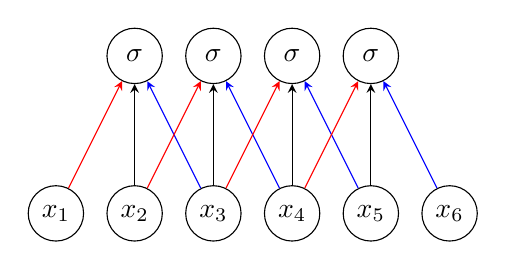
\begin{tikzpicture}[->, >=stealth, swap]
			\node [neuron] (x1) at (0,0) {$x_1$};
			\node [neuron] (x2) at (1,0) {$x_2$};
			\node [neuron] (x3) at (2,0) {$x_3$};
			\node [neuron] (x4) at (3,0) {$x_4$};
			\node [neuron] (x5) at (4,0) {$x_5$};
			\node [neuron] (x6) at (5,0) {$x_6$};
			\node [neuron] (sigma1) at (1,2) {$\sigma$};
			\node [neuron] (sigma2) at (2,2) {$\sigma$};
			\node [neuron] (sigma3) at (3,2) {$\sigma$};
			\node [neuron] (sigma4) at (4,2) {$\sigma$};
			
			\draw (x1) edge[red] (sigma1);
			\draw (x2) edge[black] (sigma1);
			\draw (x3) edge[blue] (sigma1);
			
			\draw (x2) edge[red] (sigma2);
			\draw (x3) edge[black] (sigma2);
			\draw (x4) edge[blue] (sigma2);
			
			\draw (x3) edge[red] (sigma3);
			\draw (x4) edge[black] (sigma3);
			\draw (x5) edge[blue] (sigma3);
			
			\draw (x4) edge[red] (sigma4);
			\draw (x5) edge[black] (sigma4);
			\draw (x6) edge[blue] (sigma4);
	\end{tikzpicture}
	\caption{Visual representation of a one-dimensional convolution implemented as the first layer of a convolutional neural network. The connections between the input layer and the convolutional layer are sparse in that each unit is connected only to three of six inputs. The colors of the connections indicate how the weights are shared.}
	\label{convolutional_network}
\end{figure}




\section{Summary}
In this section we have seen how to define $\mathcal{H}$ with neural networks, and we have seen how to search this space using backpropagation and gradient descent. Moreover, we have discussed regularization techniques that restrict the learning algorithm to a limited region of $\mathcal{H}$ in order to reduce the risk of overfitting. Finally, we have introduced convolutional neural networks that take advantage of convolutions as feature detectors.